\chapter{Implementation}
\label{ch:implementation}

\section{Introduction and Scope}
\label{sec:implementation-introduction-scope}

This chapter presents the implementation of the selected concept as a fully developed system. Based on the evaluation results using the \ac{wsm}, Concept B is selected for implementation, as it satisfies the majority of the defined functional, non-functional, and software platform requirements outlined in Chapter~\ref{ch:system-concept-methodology}. In particular, Concept~B enables automatic robot program generation, integrated constraint validation, and seamless operation within the drag\&bot runtime environment.

The system generates robot programs automatically using input configurations provided by the user and determines feasible solutions to execute complete sheet metal bending operations. This eliminates manual waypoint generation and function block arrangement, thereby reducing operator intervention and improving consistency and repeatability.

The implementation was developed from the requirements and concept decision described in the previous chapters. The defined requirements were translated into a modular software structure that separates configuration handling, communication, planning, validation, and execution. In practical terms, the system starts from workpiece and process parameters, the selected bend side, robot and tool settings, and the tracked sheet pose in the virtual cell. It then checks whether the initial state is valid, determines a feasible pickup orientation and grip, applies regrip or flip logic when required, and converts the resulting task sequence into robot motion and gripper commands. The output of the pipeline is therefore an executable sequence of handling and bending-related actions sent to the drag\&bot runtime through the AnyRobot interface.

The implementation is structured around four key domains. The chapter first presents the system architecture, including communication, configuration, and operator interface structures. It then describes the development and simulation environment, followed by the functional subsystems in execution order, including safety validation, orientation determination, grip planning, gripper control, regrip handling, opposite-side bending, and trajectory generation. The chapter concludes with a Failure Mode and Effects Analysis and a requirement-to-implementation traceability mapping.

The system operates entirely within the drag\&bot virtual simulation environment. Communication with the robot runtime is established through the AnyRobot interface using an authenticated WebSocket connection, ensuring compliance with \acs{sr}-01 and \acs{sr}-02. All process parameters are loaded from a central \ac{yaml} configuration file at the beginning of each execution cycle. This enables adaptation to different workpiece geometries without modifying the source code, thereby satisfying \acs{nfr}-02.

Operator input is provided through an interactive 3D sheet bending viewer integrated into the drag\&bot operator cockpit. This interface improves usability and reduces the likelihood of incorrect input selection. Ubuntu Linux is used as the development platform due to its compatibility with \acs{ros}-based systems and stable integration with the drag\&bot environment \cite{quigley2009ros}.

Figure~\ref{fig:overall-system-workflow} summarises the end-to-end execution sequence from session initialisation to bending execution. The workflow begins with configuration selection and parameter initialisation, followed by pre-execution safety validation to ensure that all operating conditions are within acceptable limits. Based on the detected sheet pose, a valid pickup orientation is determined, after which feasible grip positions are computed using constraint-based evaluation.

If direct execution is not feasible, the system automatically applies regrip strategies to achieve a reachable configuration. The validated task sequence is then converted into motion commands and executed by the robot. The process iterates over all required bending steps and includes additional handling for opposite-side operations before concluding with the final unloading stage. This structured workflow ensures deterministic execution, consistency, and repeatability across all functional subsystems within the automated bending process.

\begin{figure}[p]
    \centering
    \begin{subfigure}{\textwidth}
        \centering
        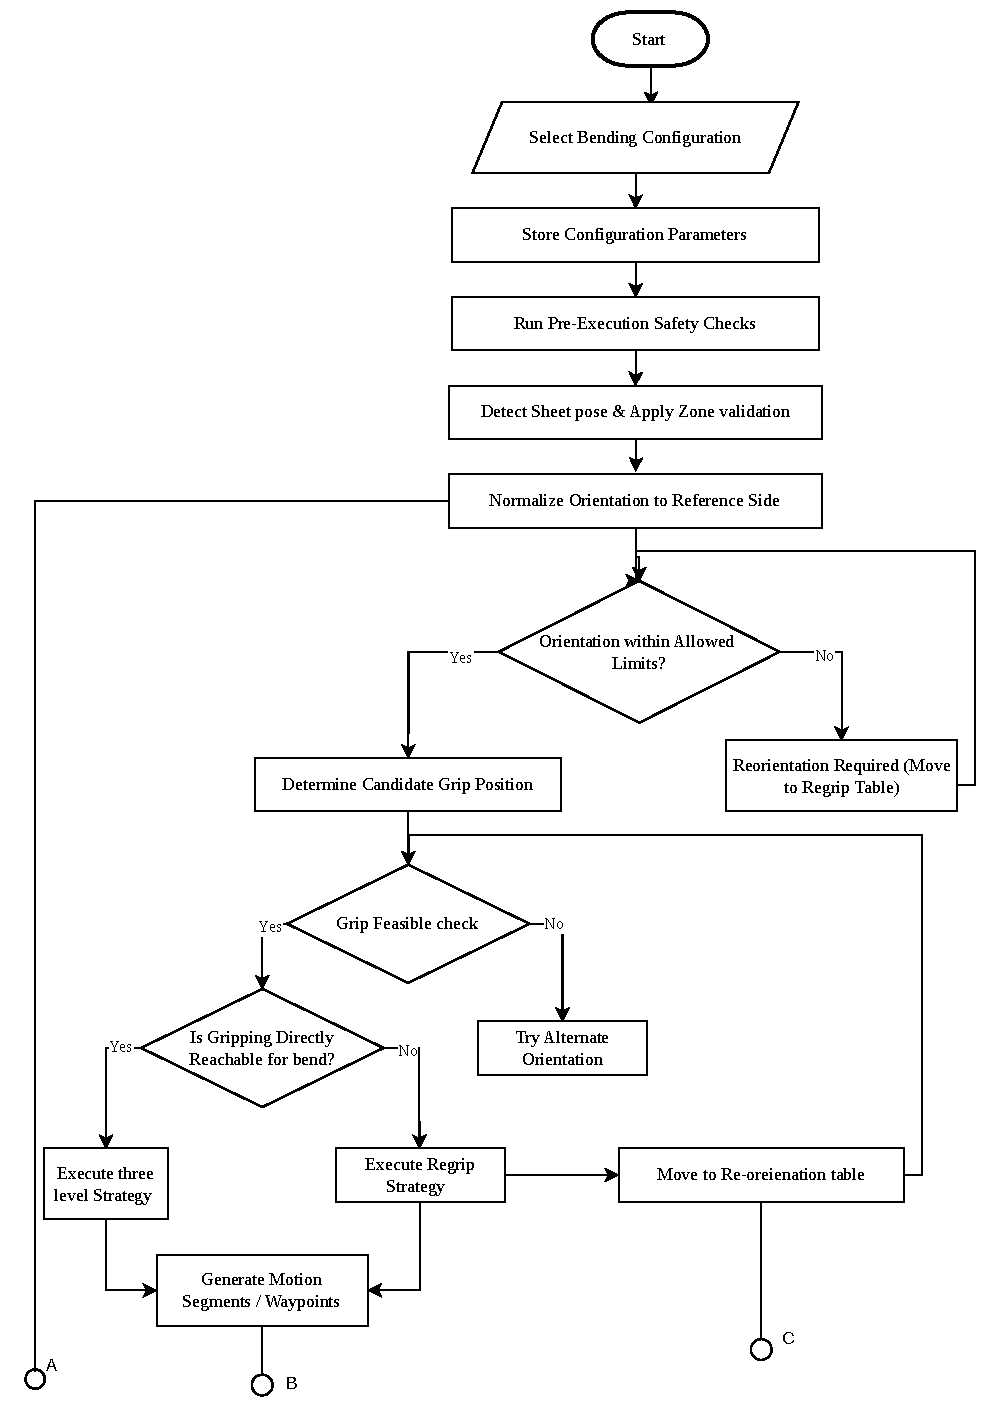
\includegraphics[width=\textwidth,height=0.38\textheight,keepaspectratio]{Flow_Diagrams/overall system 1.drawio.pdf}
        \caption{Upstream stages from configuration loading to orientation and grip planning.}
        \label{fig:overall-system-workflow-part1}
    \end{subfigure}

    \vspace{0.5em}

    \begin{subfigure}{\textwidth}
        \centering
        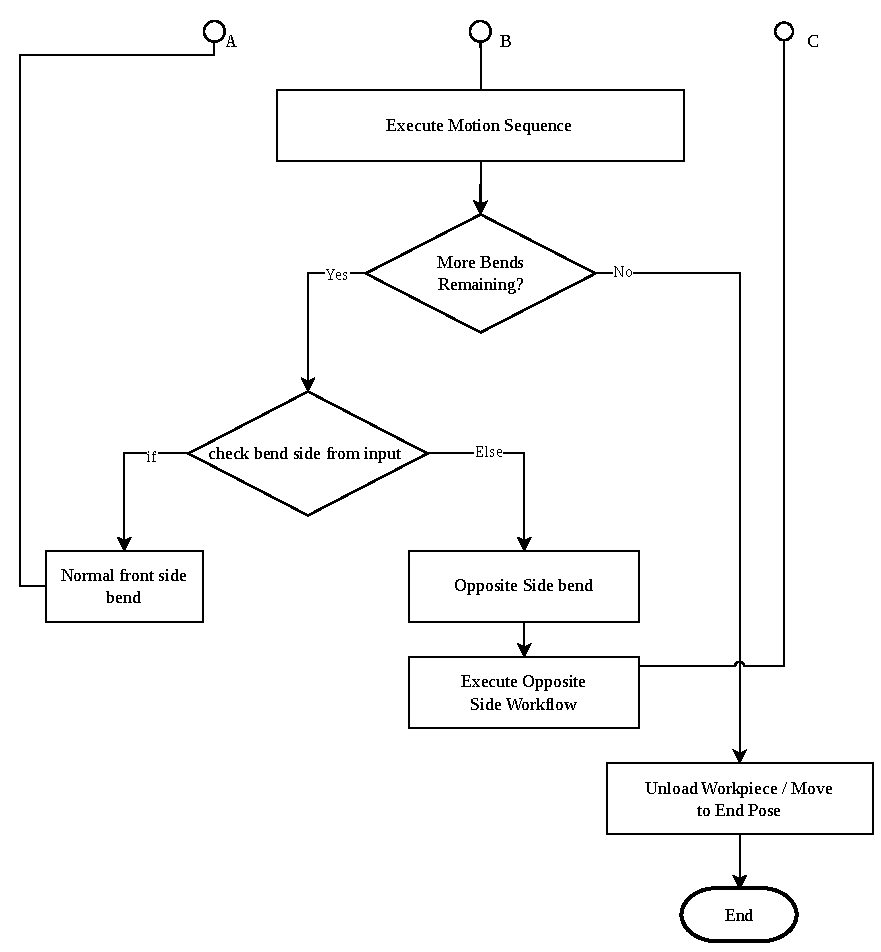
\includegraphics[width=\textwidth,height=0.38\textheight,keepaspectratio]{Flow_Diagrams/overall system 2 .drawio.pdf}
        \caption{Downstream execution stages from regrip or flip handling to trajectory execution and completion.}
        \label{fig:overall-system-workflow-part2}
    \end{subfigure}
    \caption[Complete end-to-end system workflow]{Complete end-to-end system workflow. Part~\subref{fig:overall-system-workflow-part1} shows the upstream stages, while Part~\subref{fig:overall-system-workflow-part2} shows the downstream execution stages from planning continuation to completion.}
    \label{fig:overall-system-workflow}
\end{figure}

The resulting data flow is summarised in Table~\ref{tab:ch5-end-to-end-data-flow}. The table separates the information entering each stage from the processing result produced for the next module, so that the implementation can be read as a continuous transformation from user and geometry input into executable runtime commands.

\begin{table}[htbp]
\centering
\small
\setlength{\tabcolsep}{3pt}
\renewcommand{\arraystretch}{1.08}
\begin{tabularx}{\textwidth}{C{0.8cm} Y Y Y Y}
\hline
\textbf{Step} &
\textbf{Input} &
\textbf{Processing Stage} &
\textbf{Output} &
\textbf{Next Module} \\
\hline
1 &
Workpiece geometry, bend-side selection, \ac{tcp}, gripper, and safety parameters &
Configuration and operator-input initialisation &
Structured task and configuration data &
Safety validation \\
\hline
2 &
Configuration data, fixture states, and operator start decision &
Pre-execution validation and runtime readiness checks &
Permission to continue or controlled stop &
Pose acquisition and zone classification \\
\hline
3 &
Tracked sheet pose and workspace zone &
Orientation admissibility and pickup-side validation &
Selected pickup orientation or conservative fallback &
Grip planning \\
\hline
4 &
Selected orientation, sheet geometry, and gripper parameters &
Grip candidate generation, filtering, and force validation &
Feasible grip configuration and pickup poses &
Regrip and sequence planning \\
\hline
5 &
Current workpiece pose, selected grip, and target bending pose &
Direct reachability, regrip, and opposite-side handling logic &
Validated task sequence with required handling actions &
Trajectory generation \\
\hline
6 &
Ordered task poses and handling actions &
Interpolation, kinematic validation, path reduction, and command formatting &
Executable robot motion and gripper commands &
AnyRobot runtime communication \\
\hline
\end{tabularx}
\caption{End-to-end data flow from workpiece and process input to executable robot commands.}
\label{tab:ch5-end-to-end-data-flow}
\end{table}


\FloatBarrier
%%%%%%%%%%%%%%%%%%%%%%

\section{System Architecture, Interfaces, and Configuration}
\label{sec:system-architecture}

The following section describes the software structure used to implement this pipeline before the individual planning functions are discussed.

\subsection{Layered Software Architecture and Module Responsibilities}
\label{sec:layered-architecture}

The implemented system follows a systematic layered architecture in which each module depends on the functionality provided by the underlying layer. This architectural design supports press brake automation by enabling independent testability, structured constraint evaluation, maintainability, and safe replaceability of components.

Testability is achieved by allowing modules to be evaluated using pose data and \acs{yaml}-based configuration inputs without requiring an active WebSocket connection. This enables verification of orientation classification and grip feasibility computations prior to establishing communication with the runtime environment.

Replaceability is ensured through modular separation. Individual modules can be modified or replaced without affecting the entire system, as each layer operates independently within its defined responsibility. This supports maintainability and satisfies \acs{nfr}-02.

Safety ordering is enforced by implementing validation prior to motion generation. This ensures that safety checks and kinematic feasibility evaluations are performed before execution, thereby satisfying \acs{fr}-07 and \acs{nfr}-03.

Five layers are defined within the system architecture.

Layer 1 (Input and Configuration) is responsible for acquiring all required parameters from the input file, including the operator-defined bend-side selection, before establishing the WebSocket connection.

Layer 2 (Geometry and Constraint Evaluation) performs the computation of geometric and physical constraints based on input pose data.

Layer 3 (Planning and Decision Logic) determines the overall execution strategy and coordinates the interaction between Layers 2 and 4 without directly generating motion commands. This layer prepares the execution sequence based on evaluated data.

Layer 4 (Motion Generation and Communication) serves as the interface for robot communication. It generates \ac{lin} and \ac{ptp} waypoints, converts them into \ac{json} format, and transmits them via an authenticated WebSocket connection.

Layer 5 (Safety and Validation) is implemented as an independent validation layer prior to execution. This layer identifies invalid poses and generates warnings before transmitting commands to the robot runtime.

The layer numbering describes responsibility rather than chronological execution. During runtime, validation is invoked before motion dispatch and monitoring continues during execution, while communication remains centralised in Layer~4. This distinction is important because the safety layer is architecturally separated but operationally active before and during command execution.

The layered architecture is implemented as a fixed dependency structure in which input and configuration handling, geometric evaluation, planning logic, motion generation, and safety validation remain clearly separated. This ordering ensures that validation is enforced before motion dispatch and that communication is centralised through the runtime layer.

The progression of data throughout a bending cycle follows a structured flow across the system layers. Initially, sheet geometry, bend-side selection, and tool parameters are provided as input. These inputs are processed within the constraint evaluation layer, where raw pose data is transformed into a validated pickup orientation and a feasible grip configuration.

Based on this information, an execution strategy is determined and translated into motion commands, which are transmitted to the runtime environment through the AnyRobot interface. Errors introduced at any stage may propagate through subsequent computations and affect execution outcomes.

Accurate orientation determination is critical for successful workpiece acquisition, while grip feasibility evaluation ensures stable handling during transport. During trajectory generation, a balance must be maintained between path accuracy and controller limitations, requiring controlled reduction of trajectory points while preserving motion characteristics.

\phantomsection\label{sec:module-overview}
\noindent\textbf{Module responsibilities and dependency discipline.}

The implementation consists of software modules organised across the five system layers. Table~\ref{tab:module-overview} summarises the grouped module contracts by showing what each functional group receives, what it produces, and how failure or stop conditions are handled before or during execution.

\clearpage
\begin{table}[p]
\centering
\captionsetup{font=normalsize}
\normalsize
\setlength{\tabcolsep}{4pt}
\renewcommand{\arraystretch}{1.05}

\begin{tabularx}{\textwidth}{C{0.9cm} C{1.1cm} L{3.6cm} Y}
\toprule
\textbf{No.} & \textbf{Layer} & \textbf{Module} & \textbf{Primary Responsibility} \\
\midrule
1 & L1 & Session launcher & Starts the session, loads \ac{yaml} data, and opens the 3D viewer. \\
2 & L1 & Configuration reader & Loads and validates configuration parameters. \\
3 & L5 & Safety checker & Performs operator confirmation and pre-execution safety checks. \\
4 & L2 & Zone classifier & Assigns the sheet pose to a workspace zone. \\
5 & L2 & Orientation selector & Selects a valid pickup orientation. \\
6 & L2 & Face orientation converter & Converts tracker pose data into a reference-face form. \\
7 & L2 & Grip position planner & Computes feasible grip positions under geometric constraints. \\
8 & L2 & Pickup orientation validator & Verifies tool alignment and applies corrections if needed. \\
9 & L4 & Trajectory generator & Generates waypoint sequences for executable robot motion. \\
10 & L4 & Regrip motion executor & Executes transport, release, and regrasp motions. \\
11 & L3 & Primary bending orchestrator & Coordinates the main bending workflow. \\
12 & L3 & Regrip sequencer & Determines regrip transition sequences. \\
13 & L3 & Opposite-side runner & Executes opposite-side handling when required. \\
14 & L3 & Multi-stage regrip loop & Handles repeated repositioning in complex cases. \\
15 & L3 & Post-bend unload sequencer & Controls unloading of finished workpieces. \\
16 & L4 & Waypoint data structure & Stores pose, velocity, and blending parameters. \\
17 & L4 & Digital IO handler & Controls vacuum and related input/output signals. \\
18 & L4 & WebSocket client & Manages authentication and runtime communication. \\
19 & L4 & Command type definitions & Defines motion types and \ac{json} message formats. \\
\bottomrule
\end{tabularx}

\caption{Software modules across system layers and their primary responsibilities.}
\label{tab:module_overview}
\end{table}

\clearpage

The modules exchange data as part of one execution pipeline, but their dependencies are restricted to preserve a clear separation of responsibilities. This means that modules cooperate during program generation while specific tasks, such as communication, safety validation, and motion dispatch, remain assigned to defined layers.

First, runtime communication is centralised in Layer 4. The WebSocket client and the command type definitions are the only modules that construct WebSocket messages and perform direct network communication. Modules in the other layers therefore access the runtime environment through this communication layer instead of opening their own connections. As a result, authentication handling, message formatting, and connection recovery are implemented in one place and remain consistent across all runtime interactions.

Second, safety validation is separated into Layer 5. The safety checker is executed before the runtime workflow continues and is not called directly by lower-layer planning modules during motion execution. This fixed ordering ensures that safety checks cannot be skipped, delayed, or reordered by the planning and execution logic.

Third, robot motion dispatch is centralised through the trajectory generator. All waypoint sequences are passed through this module before being transmitted to the runtime environment. This ensures that workspace constraints and singularity-related checks are applied consistently before motion execution.

After defining these dependency rules, the Layer 4 communication mechanism is described in more detail.

%%%%%%%%%%%%%%%%%%%%%%%%%%%%%%%%%%%%%%%%%%
\subsection{Runtime Communication and Configuration}
\label{sec:runtime-communication-anyrobot}

The AnyRobot interface is the drag\&bot communication interface that enables external planning software to interact with the robot runtime. In the implemented system, all runtime communication is performed through this interface, which acts as the supported external \ac{api} for drag\&bot. Through ROSBridge v2, the interface translates \ac{json} messages exchanged over a persistent WebSocket connection into native \ac{ros} operations. This allows the planning software to run in standard Python~3 without requiring a local \ac{ros} installation \cite{dragandbot_anyrobot_2025}.

The communication layer is implemented as a Python-based runtime client with structured command objects. The planning modules do not communicate with \ac{ros} directly. Instead, they pass validated motion waypoints, input-output actions, object-management requests, and operator-interaction requests to the communication layer. The runtime client serialises these requests into \ac{json} messages, transmits them through the authenticated AnyRobot WebSocket connection, and waits for the corresponding runtime response before the workflow continues.

A persistent WebSocket connection is preferred over repeated \ac{http} requests because the system must exchange commands and state information continuously during execution. WebSocket communication reduces overhead compared with repeated \ac{http} polling for real-time data exchange \cite{Pimentel2012}. Rosbridge enables non-\ac{ros} applications to communicate with \ac{ros} through socket-based interfaces \cite{Crick2017}. As illustrated in Figure~\ref{fig:communication-architecture}, the planning software communicates with the runtime through a configured endpoint of the form \texttt{ws://<runtime-ip>:<port>}. Dedicated service and topic interfaces separate motion execution, object management, gripper control, operator interaction, and execution feedback.

Table~\ref{tab:anyrobot-runtime-interfaces} summarises the principal runtime interfaces used in the implemented workflow. The \ac{yaml} configuration is not exchanged during runtime; it is loaded once during initialisation so that missing or inconsistent parameters can be detected before command transmission begins.

% ================= TABLE (FIXED POSITION) =================
\begin{table}[H]
\centering
\normalsize
\setlength{\tabcolsep}{4pt}
\begin{tabularx}{\textwidth}{L{4.2cm} L{5.2cm} Y}
\hline
\textbf{Runtime Function} & \textbf{Interface} & \textbf{Use in the Implemented Workflow} \\
\hline
Motion command dispatch & \path{/command_list} & Transmits generated \ac{lin} and \ac{ptp} waypoint sequences to the runtime environment. \\
\hline
Motion result feedback & \path{/command_result} & Returns execution results and motion status information after command dispatch. \\
\hline
Digital input-output control & \path{/robot/set_digital_ios}, \path{/robot/get_digital_ios} & Controls and queries vacuum gripper signals and related robot input-output states. \\
\hline
Object management & \path{/dnb_object_manager/...} & Queries and updates workpiece and fixture states used during attachment, detachment, and validation. \\
\hline
Operator interaction & \path{/human_interaction/request_hi} & Requests operator confirmation or warning acknowledgement through the drag\&bot interface. \\
\hline
\end{tabularx}
\caption{Principal AnyRobot runtime interfaces used by the implemented communication layer.}
\label{tab:anyrobot-runtime-interfaces}
\end{table}


% ================= FIGURE (FIXED POSITION) =================
\begin{figure}[H]
    \centering
    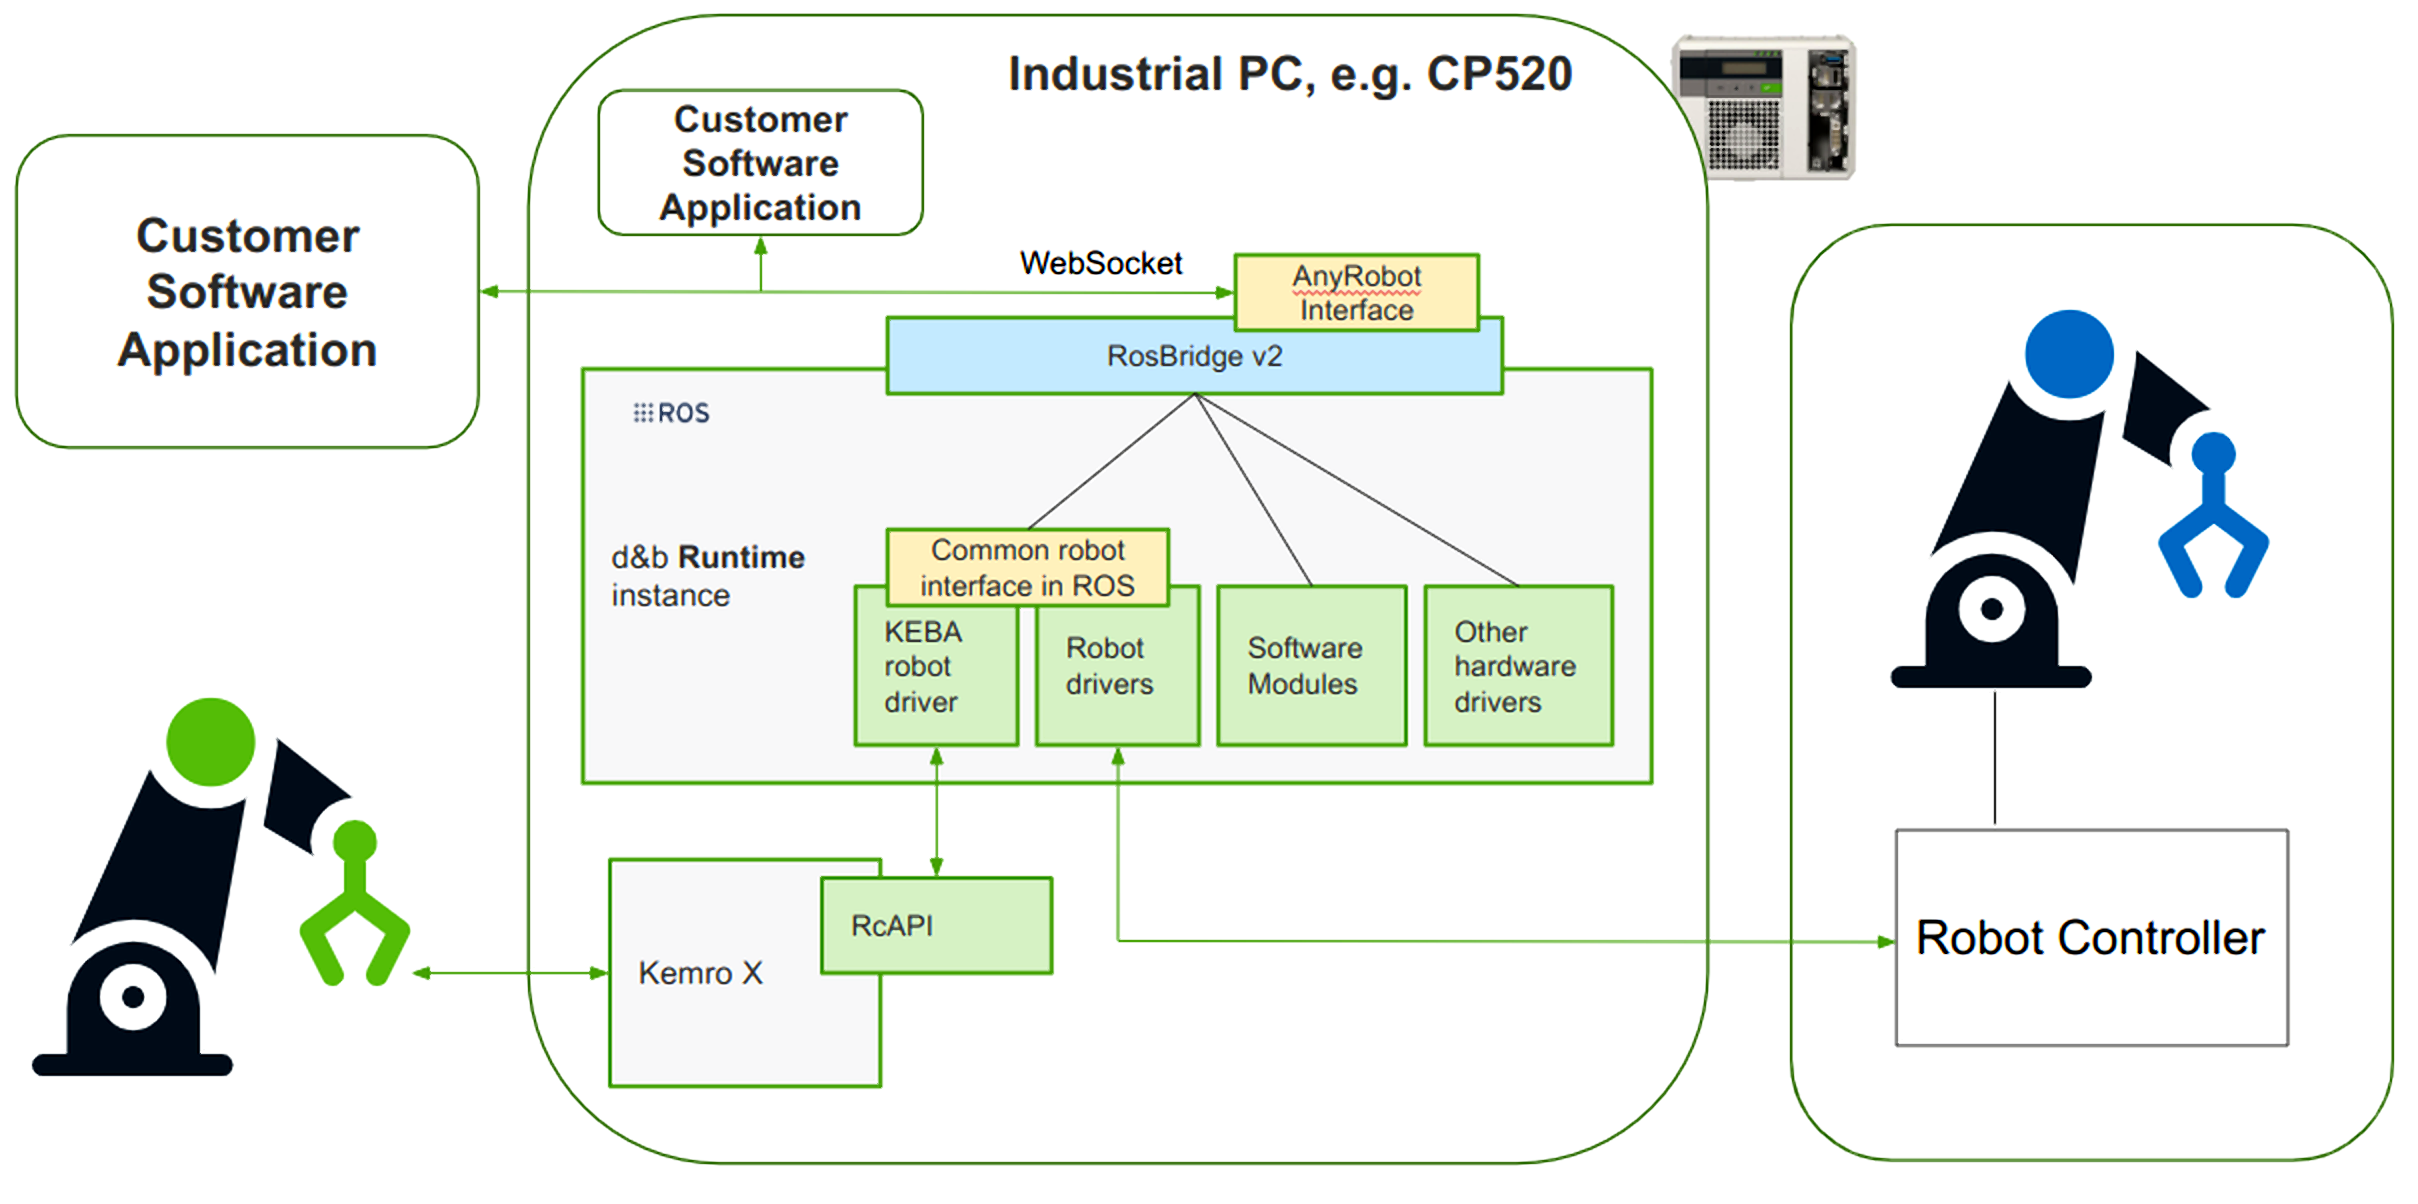
\includegraphics[width=\textwidth]{figures/communication_architecture.png}
    \caption[Communication architecture of the implemented system]{Communication architecture of the implemented system, illustrating the interaction between the planning software, the drag\&bot runtime environment, and the robot controller \cite{dragandbot_anyrobot_2025}.}
    \label{fig:communication-architecture}
\end{figure}

When the connection is established, the runtime client performs the ROSAuth handshake defined by the drag\&bot AnyRobot interface specification \cite{dragandbot_anyrobot_2025}. This step prevents unauthorised command transmission through the local WebSocket endpoint. The shared secret required for the \ac{sha512}-based authentication code is stored outside the source code as an environment variable. After authentication, planning modules exchange only validated command objects with the communication layer; the low-level message formatting remains encapsulated inside the runtime client.

Motion execution is treated as a blocking runtime interaction in the communication layer. Before dispatching a movement, the client subscribes to \texttt{/command\_result}; after the runtime returns the result code, the client releases the motion sequence and the planning workflow continues. Additional runtime supervision through an independent monitoring subprocess is described in Section~\ref{sec:operator-authorisation-runtime-monitoring}.

The implemented communication sequence is summarised in Listing~\ref{lst:runtime-command-dispatch}. The listing abstracts the runtime client behaviour to the essential steps required for authenticated command transmission, result monitoring, and controlled termination after a failed command.

\begin{lstlisting}[caption={Pseudocode for runtime command dispatch and result handling.}, label={lst:runtime-command-dispatch}]
Load runtime endpoint and authentication parameters
Open persistent WebSocket connection to AnyRobot runtime
Perform ROSAuth handshake using external secret
Subscribe to the motion result feedback topic

for each validated command group in execution_sequence do
    serialise motion and handling actions as JSON command list
    transmit command list through the runtime client
    wait for blocking result feedback

    if result code indicates failure then
        stop remaining command dispatch
        notify operator through human-interaction service
        record stop reason for evaluation
        terminate execution safely
    end if
end for

Close runtime interaction after all command groups complete
\end{lstlisting}


\FloatBarrier

\phantomsection\label{sec:configuration-architecture}
\noindent\textbf{Configuration.}
The \ac{yaml} configuration file serves as the engineering-level entry point for process-related parameters and provides a flexible mechanism for adapting the system to different workpieces without modifying the underlying source code, thereby satisfying \acs{nfr}-02. At the beginning of each session, the file is parsed once, and the resulting configuration data is stored as a dictionary that is shared across all modules in Layers 2 to 4. The structure of the file is organised into six clearly defined top-level sections, each corresponding to a specific functional aspect of the system architecture, which supports clarity and maintainability.
\ac{yaml} is selected over \ac{json} primarily due to its support for inline comments. This allows engineers to document the meaning and physical relevance of individual parameters directly within the configuration file, eliminating the need to consult external documentation. To ensure robustness and security, the configuration is loaded using a safe parsing method, which prevents the execution of unintended code in the event that the file is modified or corrupted.
A key design decision concerns the handling of spatial consistency during the regrip process. Rather than defining approach and placement poses independently, all such poses are derived relative to a single reference pose defined for the orientation table. For example, the approach position is calculated by applying a fixed vertical offset to the placement pose. This design ensures that any change in the position of the orientation table requires only a single modification within the configuration file. In contrast, storing these poses independently could introduce inconsistencies: if the table position is updated but the corresponding approach position is not, the system may execute motions based on outdated spatial data. Such inconsistencies are particularly problematic because they may not be detected during configuration validation, as each parameter remains individually valid despite being collectively incorrect.

The configuration is organised into runtime communication settings, robot and \ac{tcp} parameters, workpiece dimensions and bend-side selection, gripper parameters, motion limits, and safety thresholds. This grouping is sufficient for adapting the virtual cell to different rectangular workpieces while keeping the planning logic unchanged. A generalised \ac{yaml} example is retained as an electronic supporting file rather than reproduced in the main chapter.

While the \ac{yaml} file provides a structured and flexible way to define engineering configuration parameters, it is less suitable for normal operator interaction because the workpiece geometry and selected bend sides are not visually represented. Therefore, an operator interface with an interactive three-dimensional viewer was implemented to provide clearer visual feedback and a more convenient input method during execution.

\subsection{Operator Interface and Three-Dimensional Sheet Viewer}
\label{sec:operator-interface}

The operator interface denotes the user-facing dashboard used during execution to provide process input without editing configuration files. It combines bend-side selection, workpiece visualisation, mode selection, workflow status, and confirmation controls in a single view inside the drag\&bot Operator Cockpit. This allows the operator to inspect the intended bending input visually before automated planning begins.

Operator input for each execution cycle is provided through an interactive three-dimensional sheet bending viewer developed in this work. The viewer is implemented as a local Plotly Dash application and renders the workpiece as an interactive mesh derived from the corresponding \ac{stl} file. Presenting the sheet directly as a 3D model makes bend-side selection more intuitive than relying only on abstract side labels, while the planning system handles the underlying geometric calculations.

The viewer is embedded in the drag\&bot Operator Cockpit through a Custom URL panel, so configuration, monitoring, and execution remain within one interface. The operator-facing dashboard is shown in Figure~\ref{fig:user-interface}. The figure illustrates the embedded control panel, including bend-side selection, workflow status, mode selection, and the three-dimensional preview used for visual checking before program generation.
\begin{figure}[!htbp]
    \centering
    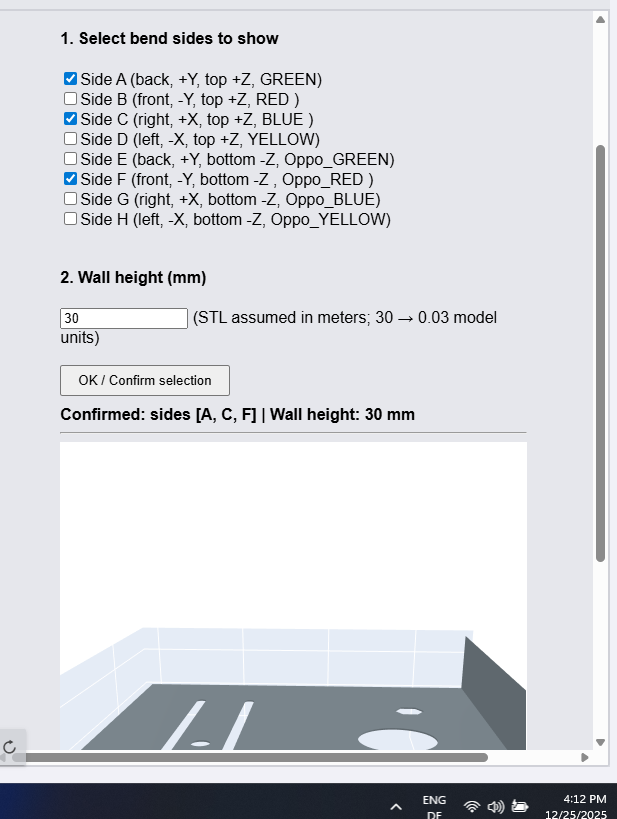
\includegraphics[width=0.50\textwidth]{figures/simulation_environment.png}
    \caption{Operator-facing sheet selection dashboard embedded in the drag\&bot Operator Cockpit, showing bend-side selection, workflow status, mode selection, and the three-dimensional workpiece preview.}
    \label{fig:user-interface}
\end{figure}
\FloatBarrier

To accommodate different levels of operator expertise, the interface is divided into basic and expert modes. Basic mode limits interaction to predefined bend-side selections and wall-height input, while expert mode exposes additional geometric, tool, and pose parameters for controlled engineering adjustment.

In parallel with user input, the system analyses the imported mesh to identify internal features such as holes. The resulting feature information is used during grip planning to exclude unsuitable regions, and the workpiece mass is estimated from material density when required for holding-force validation. Once the operator confirms the selection, the parameters are transmitted to the planning module in a structured format and further interaction is disabled to prevent configuration changes during active robot motion.
\par The complete sequence of operator interaction and system processing is summarised in Figure~\ref{fig:operator-workflow}, which illustrates the progression from initial configuration through planning, strategy selection, and final execution.


\begin{landscape}
\begin{figure}[H]
    \centering
    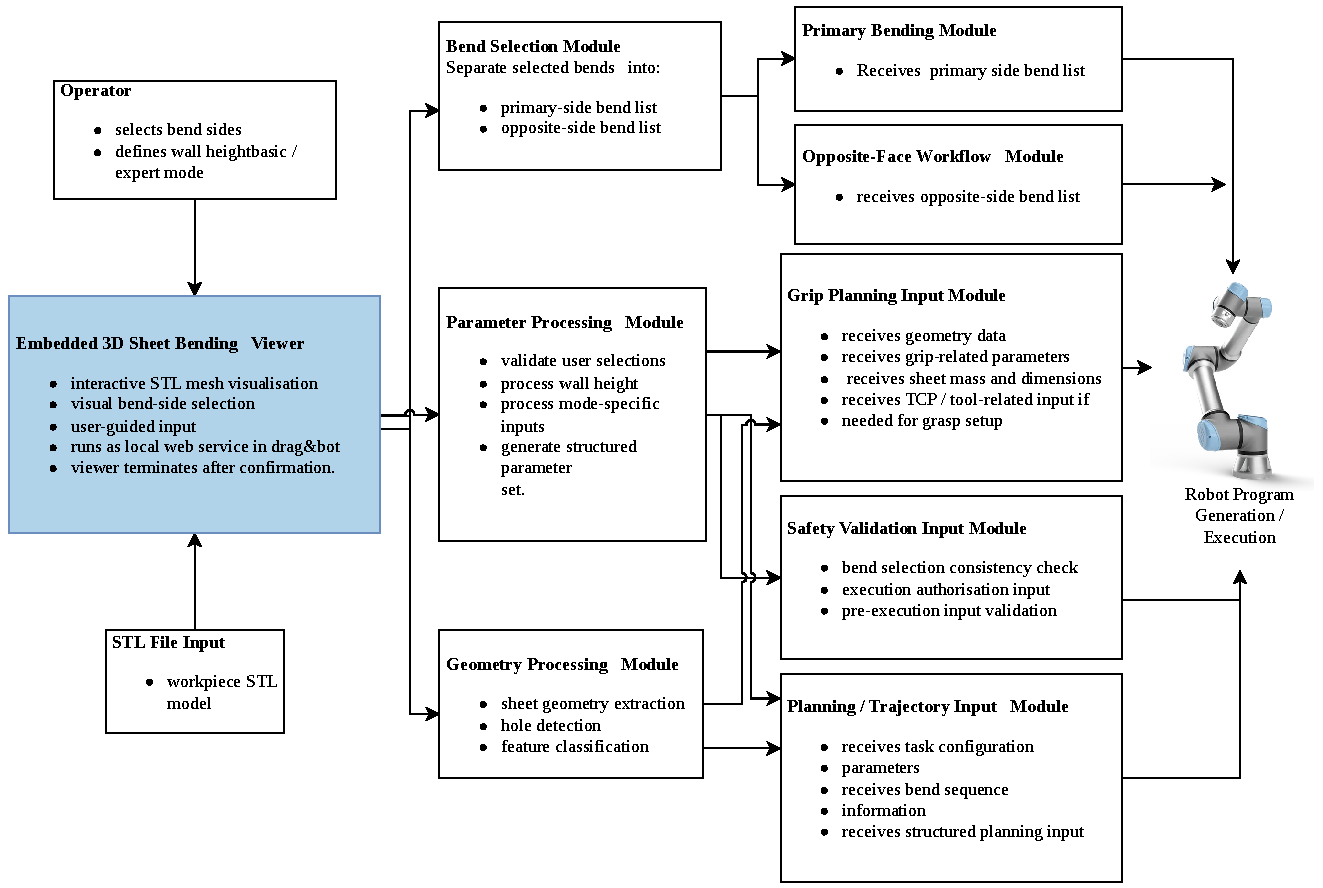
\includegraphics[width=\linewidth,height=1\textheight,keepaspectratio]{Flow_Diagrams/operator_workflow.pdf}
    \caption[Operator workflow]{Operator workflow. Every gate must be passed before the next begins. All operator interactions occur within the drag\&bot environment.}
    \label{fig:operator-workflow}
\end{figure}
\end{landscape}
\FloatBarrier

%%%%%%%%%%%%%%%%%%%%%%%%%%


\section{Simulation Environment and Pose Acquisition}
\label{sec:development-simulation-environment}

With the architectural framework established in Section~\ref{sec:system-architecture}, a controlled environment is required to execute, test, and validate the developed system prior to deployment on physical hardware. This section presents the development and simulation environment used in this work, including the drag\&bot platform, the robot model and tool configuration, and the spatial zone classification strategy used to structure the workspace.

\phantomsection\label{sec:simulation-platform}
\noindent\textbf{Simulation platform, robot model, and TCP.}

The drag\&bot platform is used as the primary environment for system development, integration, and validation. It provides a virtual robot controller together with the AnyRobot WebSocket interface, enabling the planning software to interact with the robot runtime without requiring direct access to physical equipment \cite{dragandbot_anyrobot_2025}. This supports safe testing, repeatability, and efficient iteration during development. The use of virtualised environments is consistent with current industrial trends in digital manufacturing and digital twin-based validation~\cite{Tao2021DigitalTwin}.

All modules are implemented in Python and executed within an Ubuntu-based environment alongside the drag\&bot runtime. Communication is established through a single authenticated WebSocket connection (e.g., \texttt{ws://<local-ip>:9091}), which is used for motion execution, Input/Output (IO) control, object management, and operator interaction. This unified communication structure ensures consistent behaviour across all subsystems.

All session-specific parameters are initialised at the beginning of execution and explicitly passed between modules. This avoids hidden dependencies and ensures that all components operate on consistent data, supporting modularity and maintainability.

Within this environment, the UR5e manipulator is used as the robot model. The robot provides six rotating joints, a reach of approximately 850~mm, a payload capacity of 5~kg, and a maximum joint speed of 180$^\circ$/s~\cite{universalrobots_ur5e}. These properties are suitable for the simulated press-brake handling task because the sheet must be picked, reoriented, flipped, and positioned at different approach angles during the bending sequence. The official joint range specification further supports this selection, as all joints provide a range of $\pm 360^\circ$ except the elbow joint, which provides $\pm 160^\circ$~\cite{universalrobots_ur5e}. In the implemented simulation setup, this manipulator model is therefore used to evaluate generated motion targets for reachability and feasibility before execution.

The kinematic structure of the UR5e, including the six joint frames used to describe the manipulator chain, is illustrated in Figure~\ref{fig:ur5e-kinematic-structure}. This representation is included to clarify the joint-based motion capability that is relevant for large orientation changes during sheet handling.

\begin{figure}[!htbp]
    \centering
    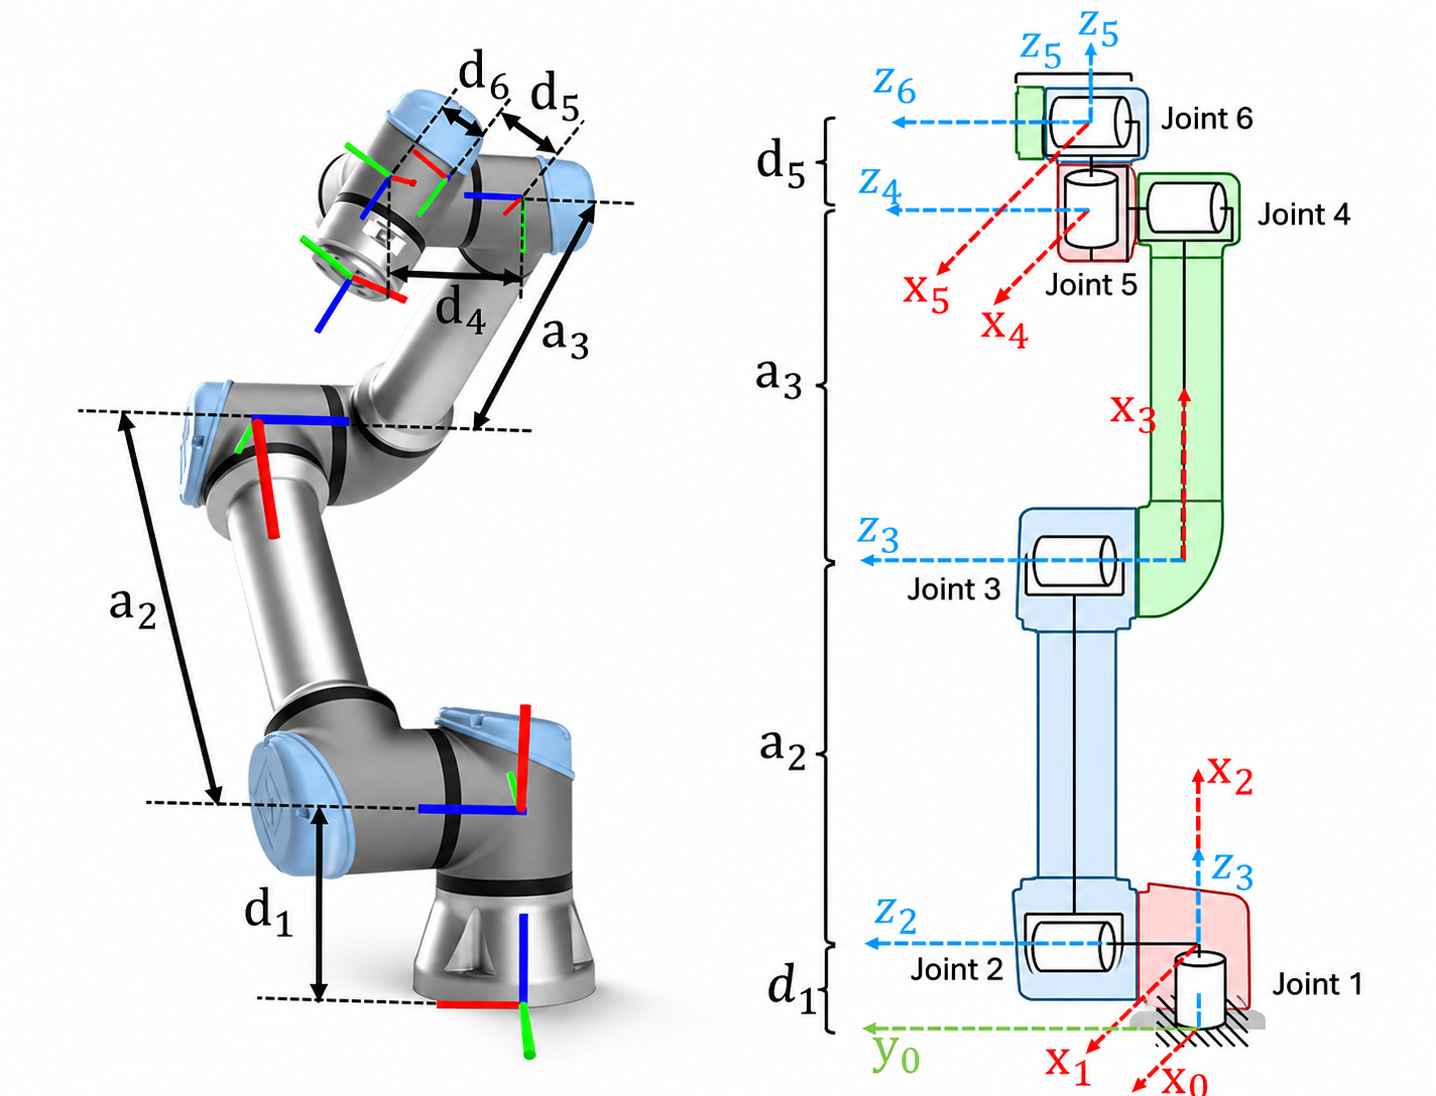
\includegraphics[width=0.5\textwidth]{figures/ur5e_robot_kinematic_structure.png}
    \caption[Kinematic structure and coordinate-frame assignment of the UR5e manipulator]{Kinematic structure and coordinate-frame assignment of the UR5e manipulator used to illustrate the six-joint robot layout \cite{zhang2025invertible}.}
    \label{fig:ur5e-kinematic-structure}
\end{figure}
\FloatBarrier

The end-effector used in the simulated cell is a two-cup vacuum gripper designed and modelled according to the company-provided tooling requirements for the project. The gripper geometry determines the position and orientation of the tool reference frame and therefore directly defines the \ac{tcp} used for all generated motion targets. In particular, the measured offset between the robot flange and the vacuum-cup contact region is represented in the configured \ac{tcp}, ensuring that planned robot poses correspond to the actual gripping position on the sheet.

The \ac{tcp} used for all motion targets is defined in the drag\&bot tool management system as \texttt{project\_3\_tcp}, in accordance with requirement \acs{sr}-03. The \ac{tcp} is specified using the ZYX Euler convention with offsets relative to the robot flange: $x = 0{,}000$~m, $y = 0{,}034$~m, $z = 0{,}194$~m, $RZ = -90{,}0^\circ$, $RY = -75{,}0^\circ$, and $RX = 0{,}0^\circ$. These parameters ensure that all generated poses remain consistent with the physical gripper configuration. The \ac{tcp} identifier is provided through the operator input, allowing future adjustments without modification of the underlying source code. The configured UR5e TCP used for the generated motion targets is shown in Figure~\ref{fig:tcp-ur5e}.

\begin{figure}[!htbp]
    \centering
    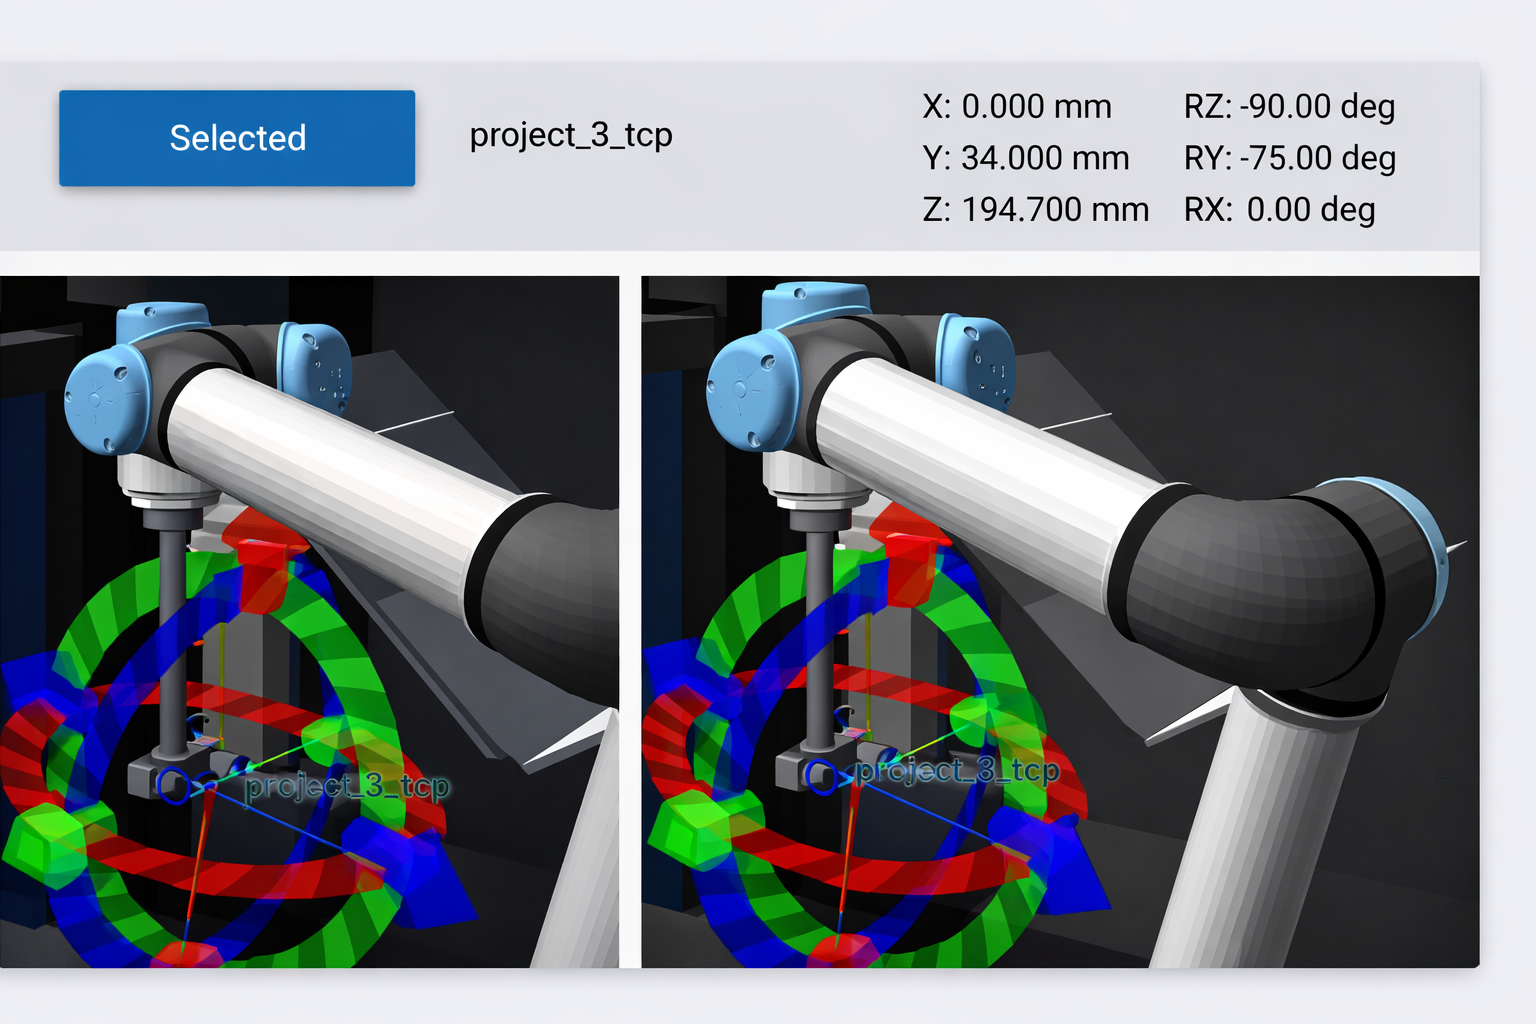
\includegraphics[width=0.6\textwidth]{figures/TCP_UR5e.png}
    \caption{Configured TCP of the UR5e with the modelled two-cup vacuum gripper used for sheet handling.}
    \label{fig:tcp-ur5e}
\end{figure}

\phantomsection\label{sec:zone-classification}
\noindent\textbf{Virtual cell layout, object pose retrieval, and spatial zone classification.}

The simulated robotic cell within the drag\&bot environment includes the robot, press brake, orientation table, flip station, vacuum gripper, and a tracked sheet object, which serves as the reference for all geometric computations. The complete virtual test environment is shown in Figure~\ref{fig:test-environment}. This operator-panel view documents the implemented cell layout used during development and validation, including the relative arrangement of the robot, press brake, handling stations, and tracked workpiece. The spatial configuration of these elements reflects the intended physical setup, ensuring that simulation results are representative of real-world operation.

\begin{figure}[!htbp]
    \centering
    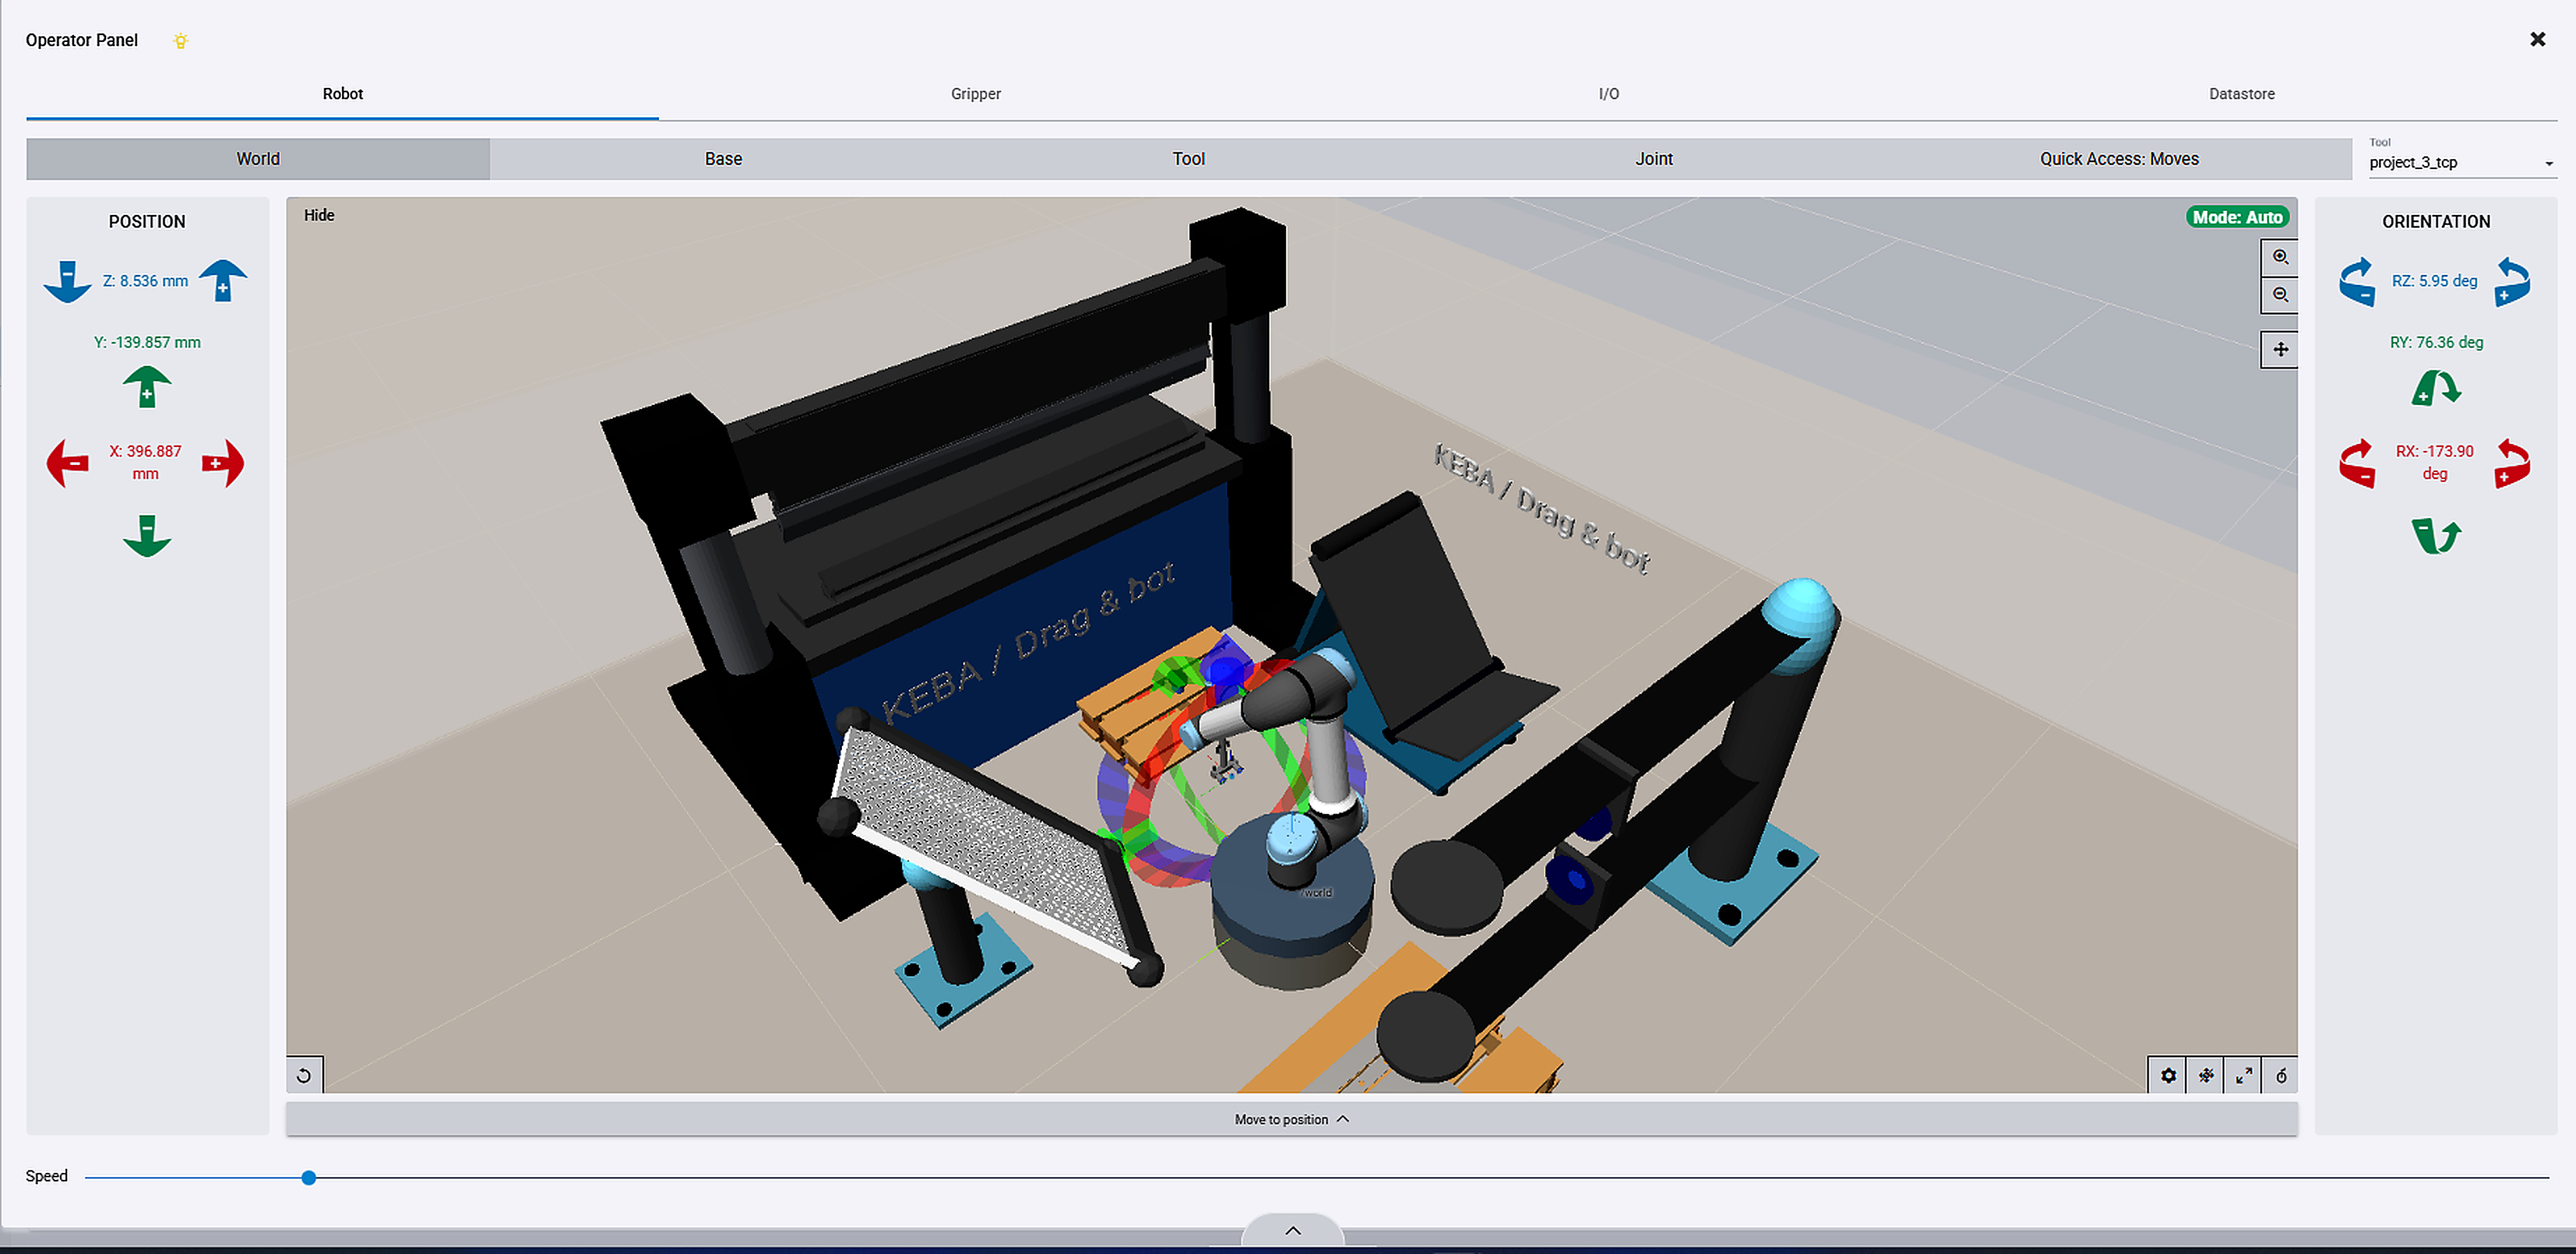
\includegraphics[width=\textwidth,height=0.55\textheight,keepaspectratio]{figures/test_environment.png}
    \caption[Virtual test environment in the drag\&bot operator panel]{Virtual test environment of the robotic press brake cell in the drag\&bot operator panel, showing the UR5e robot, press brake, handling stations, vacuum gripper, and tracked sheet object used for simulation-based development and validation.}
    \label{fig:test-environment}
\end{figure}
\FloatBarrier

In this work, object tracking refers to the retrieval of the current sheet state from the drag\&bot object manager rather than to an independent perception algorithm. In accordance with the system assumptions defined in Section~\ref{sec:system-constraints-and-assumptions}, no camera, \ac{lidar}, or external vision-based sensing is used. Instead, the simulated sheet object is maintained within the drag\&bot runtime and identified through a persistent object identifier. The planning software queries this object state through the AnyRobot interface and reads the latest available position and orientation in the robot world frame. Where available, the stored object dimensions are also read to check consistency with the configured workpiece geometry.

At the beginning of each execution cycle, the system retrieves the six-degree-of-freedom pose of the sheet from the object manager. The pose is expressed in the robot world coordinate frame, where the origin is located at the robot base. Accurate pose acquisition is a fundamental requirement in robotic manipulation systems and is widely addressed in modern robotics literature~\cite{Siciliano2016Robotics}. Based on this information, the position of the sheet centroid in the XY plane is used to classify the workpiece into one of four spatial zones.

The workspace is partitioned into four regions relative to the robot base. A centroid with negative X and positive Y corresponds to Zone~1 (rear-left), while a centroid with negative X and negative Y corresponds to Zone~2 (front-left). Positive X and positive Y correspond to Zone~3 (rear-right), and positive X with negative Y defines Zone~4 (front-right). The classification uses dead-band thresholds of $\pm 10$~mm in the X direction and $\pm 50$~mm in the Y direction around the coordinate axes. In this context, the dead band denotes a neutral region near a zone boundary in which no zone is assigned. These values are implementation parameters selected for the simulated cell rather than general robotics limits. They prevent unstable zone assignment when the sheet centroid lies close to a boundary, where small pose variations could otherwise change the sign of the coordinate and assign the workpiece to a different zone. The larger Y threshold reflects the wider separation required along the front--rear direction in the implemented cell layout.

Zones~3 and~4 lie within the primary reachable workspace of the robot and therefore allow direct execution of pickup and bending operations. In contrast, Zones~1 and~2 correspond to regions with limited reachability. In these cases, the system automatically initiates a repositioning step, moving the workpiece to an intermediate configuration within the reachable workspace before continuing execution. This ensures that all subsequent operations remain within kinematic limits without requiring operator intervention.

If the sheet centroid lies within the dead-band region defined by $|x| < 10$~mm or $|y| < 50$~mm, the classification is considered unresolved. This occurs near the coordinate axes, where small variations in tracking data may lead to inconsistent zone assignment. To prevent incorrect execution, the system terminates the current session and prompts the operator to reposition the workpiece before restarting.

Figure~\ref{fig:zone-classification} illustrates the resulting zone assignment and the neutral dead-band region around the coordinate axes.

\begin{figure}[!htbp]
    \centering
    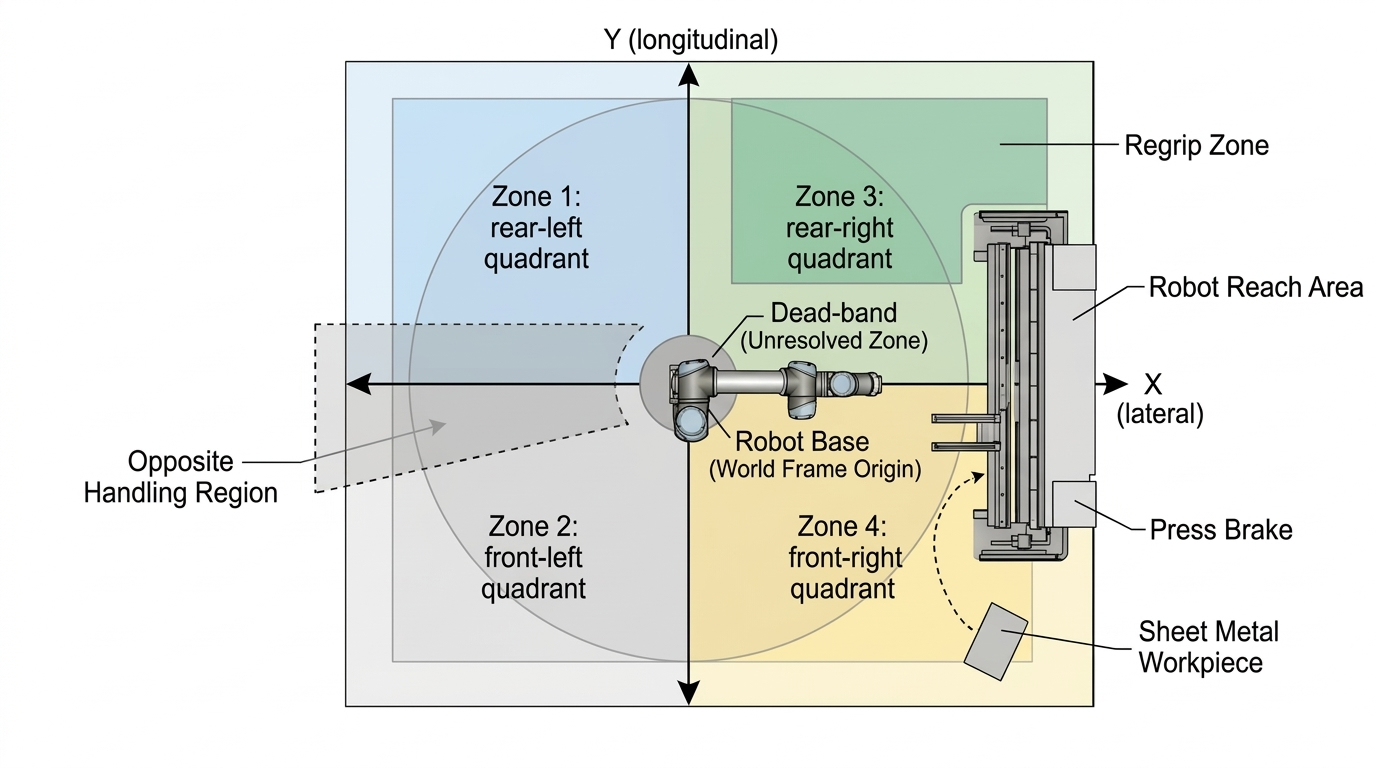
\includegraphics[width=0.8\textwidth]{figures/zone_classification.png}
    \caption{Spatial zone classification of the robot workspace based on the sheet centroid position.}
    \label{fig:zone-classification}
\end{figure}
\FloatBarrier

The implementation first applies the dead-band check and only assigns a zone when the centroid lies outside the unresolved boundary region. The signs of the remaining X and Y coordinates then determine the corresponding quadrant. This order ensures that boundary cases are rejected before a zone-dependent handling strategy is selected.

Having defined the simulation environment, robot model, \ac{tcp} configuration, object pose retrieval, and workspace segmentation strategy, the following sections describe the functional subsystems in the order of execution within a bending cycle. The workflow begins with safety validation, continues with workpiece orientation and grip planning, and then proceeds to gripper actuation, regrip or flip handling, and trajectory generation.

%%%%%%%%%%%%%%%%%%%%%%%%%%%%%
\section{Safety Validation and Runtime Monitoring}
\label{sec:pre-execution-safety-validation}

Once the virtual cell layout and coordinate references are defined, the first operational step is to check whether execution can begin safely. The input to this stage is the current object-manager state of the fixed cell references and the operator's start decision. The output is either permission to continue with planning or a controlled stop before any robot motion is issued.

Safety validation is performed prior to motion generation to ensure that unsafe conditions and infeasible configurations are identified before robot execution, in accordance with \acs{nfr}-03, \acs{nfr}-04, and \acs{nfr}-05 \cite{Siciliano2016Robotics}. The system incorporates three complementary safety mechanisms. First, a fixture pose deviation check verifies that critical objects and fixtures remain within their expected positions before execution. Second, a blocking operator confirmation dialog prevents the workflow from continuing until the operator has confirmed the setup. Third, a runtime motion error monitoring module supervises motion execution and detects command failures during operation. In addition, all trajectory waypoints are generated and verified using robot kinematics to ensure reachability and feasibility before execution, thereby preventing invalid motion commands from being issued \cite{Siciliano2016Robotics}.

\phantomsection\label{subsec:fixture-pose-deviation-validation}
\noindent\textbf{Fixture pose deviation validation.}

The fixture pose deviation check retrieves the current poses of fixed cell references from the drag\&bot object manager and compares them with reference poses obtained during initial cell calibration. The monitored elements include the press brake reference, the finished-part placement positions on the regrip table, and the placement and attachment references at the flip station. These elements are treated as fixed references within the planning system, as grip positions, trajectory waypoints, and placement operations are computed under the assumption that their positions remain unchanged. If one of these references is moved, the corresponding position parameters in the configuration or operator interface must be updated before execution. Otherwise, the generated motion targets may remain geometrically valid in software while no longer matching the physical or simulated cell layout.

The active workpiece is treated differently from these fixed references. Since the sheet may be placed in different positions and orientations before a bending cycle begins, its pose is not compared against a single fixed reference pose. Instead, the system verifies that a valid sheet pose is available from the object manager and passes this pose to the zone classification and workpiece orientation strategy described in Sections~\ref{sec:zone-classification} and~\ref{sec:workpiece-orientation}. This separation is necessary because arbitrary workpiece placement is part of the intended workflow, while movement of fixed cell references indicates an inconsistent setup.

Each fixed reference is evaluated using both positional and orientation criteria. The positional deviation is computed using the standard three-dimensional Euclidean distance according to Equation~\ref{eq:fixture-position-deviation}~\cite{OpenStaxCalculusVolume3}:

\begin{equation}
\Delta_{pos} = \sqrt{(\Delta x)^2 + (\Delta y)^2 + (\Delta z)^2}
\label{eq:fixture-position-deviation}
\end{equation}

In Equation~\ref{eq:fixture-position-deviation}, $\Delta x$, $\Delta y$, and $\Delta z$ denote the differences between the current and reference positions along the three Cartesian axes. The resulting value $\Delta_{pos}$ is therefore the three-dimensional distance between the expected reference position and the currently reported position.

The orientation deviation is defined in this implementation by Equation~\ref{eq:fixture-orientation-deviation}:

\begin{equation}
\Delta_{ang} = \max\left(|\Delta RZ|, |\Delta RY|, |\Delta RX|\right).
\label{eq:fixture-orientation-deviation}
\end{equation}

In Equation~\ref{eq:fixture-orientation-deviation}, $\Delta RZ$, $\Delta RY$, and $\Delta RX$ denote the differences between the current and reference orientations about the corresponding axes. The maximum absolute value is used because a large deviation around any one axis is sufficient to make the reference pose unreliable for planning.

A fixture is considered out of tolerance when $\Delta_{pos}$ exceeds 5~mm or $\Delta_{ang}$ exceeds 0{,}10~rad (5{,}7$^\circ$). The positional threshold is selected to remain below the minimum clearance used in grip planning. This ensures that fixture misalignment does not produce misleadingly valid grip configurations. The angular threshold corresponds to the minimum deviation that would affect the accuracy of vacuum cup contact on the sheet surface.

If one or more fixtures exceed the defined thresholds, the system generates a structured warning listing all affected fixtures together with their measured positional and angular deviations. This warning is presented through a blocking \ac{hi} dialog titled \textit{Fixture position warning}, allowing the operator to either proceed with explicit acknowledgement or cancel execution for further inspection. The operator's decision is recorded, ensuring that responsibility for accepting out-of-tolerance conditions remains with the human operator.

If a fixture is not detected in the object manager response, it is treated as missing and automatically flagged as a validation failure.

\phantomsection\label{sec:operator-authorisation-runtime-monitoring}
\noindent\textbf{Operator authorisation and runtime error monitoring.}

The operator confirmation dialog is positioned as the first step in the planning orchestrator startup sequence, preceding all subsequent processes including fixture validation, visualisation, and motion execution. The dialog enforces a mandatory decision: either initiate the automated workflow or cancel execution. The orchestrator does not proceed until a response is received from the \acs{hi} service, ensuring that execution cannot begin without explicit operator authorisation. If the operator selects cancel, the process terminates without issuing any command to the robot runtime.

Although runtime monitoring becomes active during robot motion, it is described in this section because it belongs to the same safety layer as the pre-execution checks.

In addition to pre-execution validation, runtime supervision is implemented through a motion error monitoring module operating as a background subprocess. This component subscribes to the \texttt{/command\_result} \ac{ros} topic via an independent WebSocket connection, enabling continuous monitoring of execution outcomes without interrupting the main command flow. When a non-zero result code is detected, indicating a motion execution failure, the system immediately triggers a modal \acs{hi} notification to inform the operator.

The monitoring module does not directly interrupt the execution pipeline. Instead, it provides immediate feedback through the \acs{hi} interface and requires operator acknowledgement before further interaction is permitted. This ensures that execution anomalies are not overlooked while maintaining operator authority over subsequent decisions.

Together, these mechanisms establish a layered safety structure. Pre-execution validation ensures safe initial conditions, while runtime monitoring provides immediate feedback on execution failures. Both mechanisms utilise the drag\&bot \acs{hi} service, ensuring a consistent and controlled interface for safety-related interactions. With these safeguards in place, the subsequent section addresses the workpiece orientation strategy.


%%%%%%%%%%%%%%%%%%%%%%%%%%%%%%%%%

\section{Orientation and Grip Planning}
\label{sec:workpiece-orientation}

Following safety validation, the first geometric planning step in each bending cycle is the determination of a valid pickup orientation for the sheet. The input to this stage is the tracked sheet pose and the active workspace zone. The output is a validated pickup orientation that is passed to grip planning. This step is required because the sheet may be placed in arbitrary orientations within the workspace, while only a subset of these orientations is kinematically feasible for the target bending operation.

\subsection{Zone-Based Orientation Admissibility and Pickup Validation}
\label{sec:zone-based-rz-admissibility}
\label{subsec:pickup-orientation-validation}

Before grip planning is performed, the tracked sheet pose obtained from the object manager is checked from two complementary viewpoints. First, the in-plane rotation of the sheet must be reachable from the current workspace zone. Second, the vacuum gripper must approach the correct sheet surface so that the suction cups can establish contact.

Both checks are required because the sheet may be placed in different orientations, and a detected pose may be geometrically valid but still unsuitable for pickup if the yaw angle is outside the reachable range or if the tool frame is oriented towards the wrong side of the sheet. In the latter case, the suction cups may not contact the sheet correctly, which can lead to failed gripping, incorrect attachment in the simulation model, or invalid motion targets in the following planning stages.

The admissible range of sheet rotation about the Z-axis is defined by a zone-dependent window $[RZ_{\min}, RZ_{\max}]$. This constraint reflects the limited rotational capability of the robot end-effector within different regions of the workspace \cite{Siciliano2016Robotics}. Only the rotation about the Z-axis is used for this admissibility window because it represents the in-plane orientation of the sheet within the horizontal workspace. This yaw angle determines whether the robot can approach the selected sheet side from the current zone without exceeding its reachable orientation range. Since the reachable orientation range varies with the spatial position of the sheet, zone classification is performed prior to orientation evaluation. The values $RZ_{\min}$ and $RZ_{\max}$ are predefined admissibility limits for each workspace zone. They are established during system setup by evaluating the reachable sheet yaw range in the simulated cell with the configured robot, \ac{tcp}, gripper, and surrounding stations. These limits are then stored in the configuration and are not recalculated during execution. If a candidate orientation falls outside the configured range, it is treated as not admissible and the next level of the orientation strategy is evaluated. This prevents the selection of geometrically valid but unreachable poses.

The rotations about the X- and Y-axes are evaluated in the same validation stage to verify the pickup side. These angles describe the tilt of the tool frame relative to the sheet surface, while the corresponding direction check indicates whether the tool Z-axis points towards or away from the required contact side. If the evaluated direction does not correspond to the required approach side, the corrective transformation in Equation~\ref{eq:zone-based-opposite-orientation} is applied:

\begin{equation}
RZ' = \mathrm{wrap}(RZ + 180^\circ), \quad
RY' = -RY, \quad
RX' = \mathrm{wrap}(RX + 180^\circ)
\label{eq:zone-based-opposite-orientation}
\end{equation}

In this transformation, $RZ$ is shifted by $180^\circ$ to rotate the in-plane approach direction, while $RY$ is mirrored and $RX$ is shifted by $180^\circ$ to obtain an equivalent pose from the opposite side of the sheet. The function $\mathrm{wrap}(\cdot)$ normalises the resulting angle to the configured angular range. The pickup position itself is not changed; only the orientation is corrected so that the gripper approaches the sheet from the valid side.

\subsection{Three-Level Orientation Selection Strategy}
\label{sec:three-level-orientation-selection-strategy}

After zone-based admissibility and pickup-side validation, the system must still determine which equivalent tool orientation should be used for the detected workpiece pose. This decision is required because the \ac{tcp} is fixed relative to the two-cup vacuum gripper shown in Figure~\ref{fig:tcp-ur5e}. When the sheet is placed with a different in-plane orientation, the required \ac{tcp} orientation changes accordingly. Some of these orientations may be outside the reachable range of the robot for the current workspace zone, while others may orient the suction cups towards an unsuitable side of the sheet. Therefore, the detected orientation cannot always be forwarded directly to grip planning.

To automate this decision with respect to the tracked workpiece position and orientation, a three-level selection strategy is applied. The levels are evaluated sequentially, and execution terminates as soon as a valid orientation satisfying admissibility constraints is identified. This improves robustness while prioritising geometrically consistent and kinematically feasible configurations.

The workpiece is defined using four reference faces established during system commissioning, each associated with a fixed angular offset about the sheet's local vertical axis ($0^\circ$, $180^\circ$, $+90^\circ$, $-90^\circ$). These offsets allow the system to normalise arbitrary orientations into a consistent reference frame.

In this context, a reference face denotes a predefined side of the rectangular sheet that is used as an orientation reference for pickup planning. It is not a separate physical object, but a selected sheet-side orientation defined during system setup. The reference face is chosen because its associated pickup orientation provides favourable reachability for the configured UR5e \ac{tcp} and the two-cup vacuum gripper. It therefore represents the preferred direct pickup orientation whenever the tracked workpiece pose can be transformed into this frame and still satisfies the admissibility checks described above.

\noindent\textbf{Level 1: Reference-face equivalent orientation.}

At the highest priority level, the tracked orientation is converted into a reference-face equivalent by removing the face-specific offset according to Equation~\ref{eq:bend-face-corrected-rotation}:

\begin{equation}
R_{\text{new}} = R_{\text{raw}} \cdot R_z(-d_{\text{face}})
\label{eq:bend-face-corrected-rotation}
\end{equation}

In this equation, $R_{\text{raw}}$ denotes the tracked orientation of the sheet, and $d_{\text{face}}$ denotes the angular offset of the selected reference face. The rotation $R_z(-d_{\text{face}})$ is applied about the local Z-axis to remove this face offset from the detected pose. The result, $R_{\text{new}}$, is the reference-face equivalent orientation that is then checked against the zone-dependent admissibility window.

The corrected rotation matrix is then converted into ZYX Euler angles using standard rotation-matrix decomposition \cite{Siciliano2016Robotics,lynch2017modern}. The resulting angles are denoted as $RZ$, $RY$, and $RX$ and are used for the admissibility and pickup-side checks.

After this transformation, Level 1 is accepted only if the resulting orientation satisfies the validation conditions introduced above. The computed $RZ$ must lie within the zone-specific admissibility window, expressed as $RZ_{\min} \leq RZ \leq RZ_{\max}$, and the corresponding tool orientation must remain valid for pickup from the required sheet side. If either condition is not satisfied, the reference-face equivalent orientation is considered unsuitable for execution, and the strategy proceeds to Level 2. When both conditions are satisfied, this orientation is selected. This level is preferred because it ensures consistent reference alignment and reduces trajectory complexity.

\noindent\textbf{Level 2: Detected-pose evaluation.}

If Level 1 fails, the raw tracked pose obtained from the object manager is evaluated directly. This level uses the detected workpiece position and orientation as the pickup candidate, but only if the same pickup-side validation and zone-based reachability checks are satisfied. This accounts for cases where the initial sheet placement is already feasible and avoids unnecessary transformations. If the raw $RZ$ lies within the admissibility window and the pickup orientation remains valid, the detected pose is selected. Otherwise, the strategy proceeds to the fallback level.

\noindent\textbf{Level 3: Inverted-pose fallback.}

If neither Level 1 nor Level 2 satisfies the admissibility condition, the strategy generates an inverted-pose fallback. This fallback is required because some workpiece placements cannot be reached using either the preferred reference-face orientation or the raw detected orientation, even though an opposite approach direction may still provide a possible pickup candidate. In this context, the inverted pose does not change the sheet position. It changes only the tool orientation so that the gripper is evaluated from an opposite orientation candidate, as described by Equation~\ref{eq:fallback-opposite-orientation}:

\begin{equation}
RZ' = \mathrm{wrap}(RZ \pm 180^\circ), \quad
RY' = -RY, \quad
RX' = -RX
\label{eq:fallback-opposite-orientation}
\end{equation}

In this fallback transformation, the in-plane angle $RZ$ is rotated by $180^\circ$ to test the opposite approach direction, while $RY$ and $RX$ are mirrored to form the corresponding tool orientation. The function $\mathrm{wrap}(\cdot)$ keeps the resulting in-plane angle within the configured angular range. This expands the set of possible pickup orientations when the primary checks fail, but it is not treated as equivalent to a fully validated Level 1 or Level 2 result. Since this fallback is selected only after the confirmed alternatives have failed, it is marked as \textit{admissibility not confirmed}. This status is propagated to downstream planning modules so that the pose can be handled conservatively rather than assumed to be a fully confirmed orientation.

The implemented decision sequence follows the three levels described above. The system first corrects an invalid pickup side when necessary, then evaluates the reference-face equivalent orientation. If this fails, the detected pose is checked directly. Only when both confirmed alternatives fail is the inverted fallback selected and marked as \textit{admissibility not confirmed}.

Listing~\ref{lst:orientation-selection} provides the corresponding implementation-level control flow. It shows how the detected sheet pose is converted into a selected orientation result before the grip planner is called.

\begin{lstlisting}[caption={Pseudocode for three-level orientation selection.}, label={lst:orientation-selection}]
Read tracked sheet pose from drag&bot object manager
Classify sheet centroid into the configured workspace zone
Correct pickup side if the gripper would approach an invalid face

Generate Level 1 reference-face equivalent orientation
if Level 1 satisfies zone and pickup admissibility then
    select Level 1 orientation as confirmed result
else
    Test Level 2 using the detected sheet orientation directly
    if Level 2 satisfies zone and pickup admissibility then
        select Level 2 orientation as confirmed result
    else
        Generate Level 3 inverted fallback orientation
        select fallback orientation with conservative status flag
    end if
end if

Forward selected orientation and status to grip planning
\end{lstlisting}


\noindent\textbf{Strategy outcome.}

The proposed strategy is designed to determine a valid pickup orientation where the defined constraints allow it while prioritising kinematic feasibility and geometric consistency. Level 1 represents the preferred direct pickup orientation for the subsequent bending flow. If this orientation is not available, the detected pose is evaluated in Level 2 to determine whether the workpiece can still be picked directly from its current placement.

If neither the reference-face equivalent orientation nor the detected pose satisfies the validation conditions, the fallback orientation from Level 3 is treated as a handling candidate rather than a fully confirmed bending pose. In this case, the workpiece can be transferred to the reorientation table, where it is placed in a more favourable pose before the bending sequence continues.

By integrating admissibility constraints with this structured fallback mechanism, the method directly supports pre-execution validation and reduces the likelihood of infeasible motion generation. The selected orientation is then passed to the grip planning stage, where feasible suction-cup positions are calculated for the validated tool approach.

\subsection{Grip Position Planning and Feasibility Validation}
\label{sec:grip-planning}

After a valid pickup orientation has been selected, the system must determine where the vacuum gripper can safely contact the sheet. The input to this stage is the validated pickup orientation, the workpiece geometry, and the configured two-cup gripper parameters. The output is a feasible grip configuration together with the approach, attachment, and retreat poses required for subsequent handling. This step is required because a geometrically reachable pickup orientation alone does not guarantee that the suction cups can be placed on stable, continuous, and load-bearing regions of the sheet.

\phantomsection\label{subsec:sheet-geometry-holes}
\noindent\textbf{Workpiece geometry and feasible contact regions.}

The workpiece is represented as a planar sheet with length, width, thickness, and mass obtained from the configuration. If the mass is not specified directly, it is estimated from the sheet volume and the configured material density. These parameters define the physical basis for grip planning, since both the available contact area and the required holding force depend on the sheet dimensions and mass.

The outer sheet boundary defines the maximum possible gripping area. Internal features, such as holes extracted from the \ac{stl} model, are excluded from this area because a suction cup cannot form a reliable seal over a discontinuity. Each detected hole is represented by its centre position and radius in the sheet coordinate frame. A buffer is added around these regions so that selected cup positions maintain a safe distance from feature edges. The result is a set of feasible contact regions that can be used for candidate generation.

\phantomsection\label{subsec:grip-candidate-search}
\noindent\textbf{Grip candidate generation and geometric filtering.}

Candidate suction-cup positions are generated using a grid-based search over the feasible sheet surface. The search begins with a coarse discretisation to identify usable regions and is then refined around promising areas to improve placement accuracy. Additional candidate positions are also evaluated near hole boundaries so that the available surface area can be used effectively without violating clearance requirements.

Each candidate is checked against geometric constraints before physical force validation is performed. The cup centre must remain inside the sheet boundary, satisfy the minimum edge clearance, avoid the buffered hole regions, and comply with the spacing requirements of the two-cup gripper. For the two-cup configuration, candidates are evaluated as pairs so that the distance between the suction cups provides a stable grip span across the workpiece.

After geometric filtering, only physically possible cup placements remain. These candidates are then passed to the vacuum holding force validation stage. This ordering ensures that the force model is applied only to candidate configurations that are already valid from a geometric point of view.

\phantomsection\label{subsec:vacuum-force-validation}
\noindent\textbf{Vacuum holding force validation and final selection.}

For each remaining grip candidate, the system evaluates whether the available vacuum force is sufficient to hold the sheet during handling. The contact area of one suction cup is calculated from the cup diameter using the standard circle-area relation according to Equation~\ref{eq:cup-area}:

\begin{equation}
A_{\text{cup}} = \pi \left(\frac{d_{\text{cup}}}{2}\right)^2
\label{eq:cup-area}
\end{equation}

Here, $d_{\text{cup}}$ is the suction cup diameter, and $A_{\text{cup}}$ is the effective contact area of one cup. In this thesis, vacuum feasibility is evaluated using an adapted conservative model based on standard vacuum-gripper force principles \cite{vacuum_handling_standard}. The model estimates the available holding force from the pressure difference and suction cup area, and compares it against a safety-factor-weighted resultant load that combines gravitational and inertial effects \cite{VacuumGripperModeling}. The total available holding force generated by $n$ suction cups is expressed in Equation~\ref{eq:vacuum-force}, following the standard vacuum-force relation reported for vacuum grippers~\cite{VacuumGripperModeling}:

\begin{equation}
F_{\text{vacuum}} = n \cdot \Delta P \cdot A_{\text{cup}} \cdot \eta
\label{eq:vacuum-force}
\end{equation}

In this expression, $n$ is the number of active suction cups, $\Delta P$ is the pressure difference, and $\eta$ represents efficiency losses due to leakage, surface condition, and imperfect sealing. The required holding force is calculated using the adapted vacuum-handling load formulation in Equation~\ref{eq:required-force}~\cite{vacuum_handling_standard}:

\begin{equation}
F_{\text{required}} = SF \cdot m \cdot \sqrt{a_{xy}^2 + (g + a_z)^2}
\label{eq:required-force}
\end{equation}

Here, $SF$ is the safety factor, $m$ is the sheet mass, $g$ is gravitational acceleration, and $a_{xy}$ and $a_z$ represent the expected horizontal and vertical acceleration components during handling. A grip candidate is accepted only if the available holding force is greater than or equal to the required holding force:

\begin{equation}
F_{\text{vacuum}} \geq F_{\text{required}}
\label{eq:vacuum-feasibility-criterion}
\end{equation}

Candidates satisfying both the geometric constraints and the holding force criterion are ranked using a scoring function. The score favours positions with sufficient edge clearance, distance from internal features, and stable spacing between the two suction cups. The highest-scoring configuration is selected as the final grip position.

Based on this selected configuration, the system derives three key pickup poses: the approach pose, the attachment pose, and the retreat pose. These poses define how the gripper moves towards the sheet, establishes contact, and leaves the pickup area after attachment. The complete grip planning workflow is summarised in Listing~\ref{lst:grip-selection} and illustrated in Figure~\ref{fig:grip-planning-flowchart}.

%%%%%  ALG   %%%%%
\FloatBarrier
\begin{lstlisting}[caption={Pseudocode for grip candidate search and selection.}, label={lst:grip-selection}]
Load sheet geometry and grip-planning parameters
Generate candidate grip positions using coarse-to-refined grid-based search
Add supplemental candidates near hole boundaries while respecting clearance buffers
Exclude candidates violating edge-clearance constraints
Exclude candidates overlapping with hole regions and buffer zones

if no feasible candidates remain then
    terminate grip planning
end if

if two-cup configuration is required then
    form candidate pairs
    exclude pairs violating minimum spacing constraints
end if

Validate feasible configuration(s) using the vacuum holding force criterion
Score remaining configuration(s) based on geometric suitability
Select the highest-scoring grip configuration
Compute approach, attachment, and retreat waypoints (A1, B1, R1)
Forward selected grip result to trajectory generation
\end{lstlisting}

\FloatBarrier

%%%%%%% FLOW DIAGRAM %%%%%%%
Figure~\ref{fig:grip-planning-flowchart} illustrates the complete grip planning pipeline, including force validation, candidate generation, constraint filtering, scoring, and waypoint derivation. The workflow is split into Part~\subref{fig:grip-planning-flowchart-part1} and Part~\subref{fig:grip-planning-flowchart-part2} for readability.

\begin{figure}[p]
    \centering
    \begin{subfigure}{\textwidth}
        \centering
        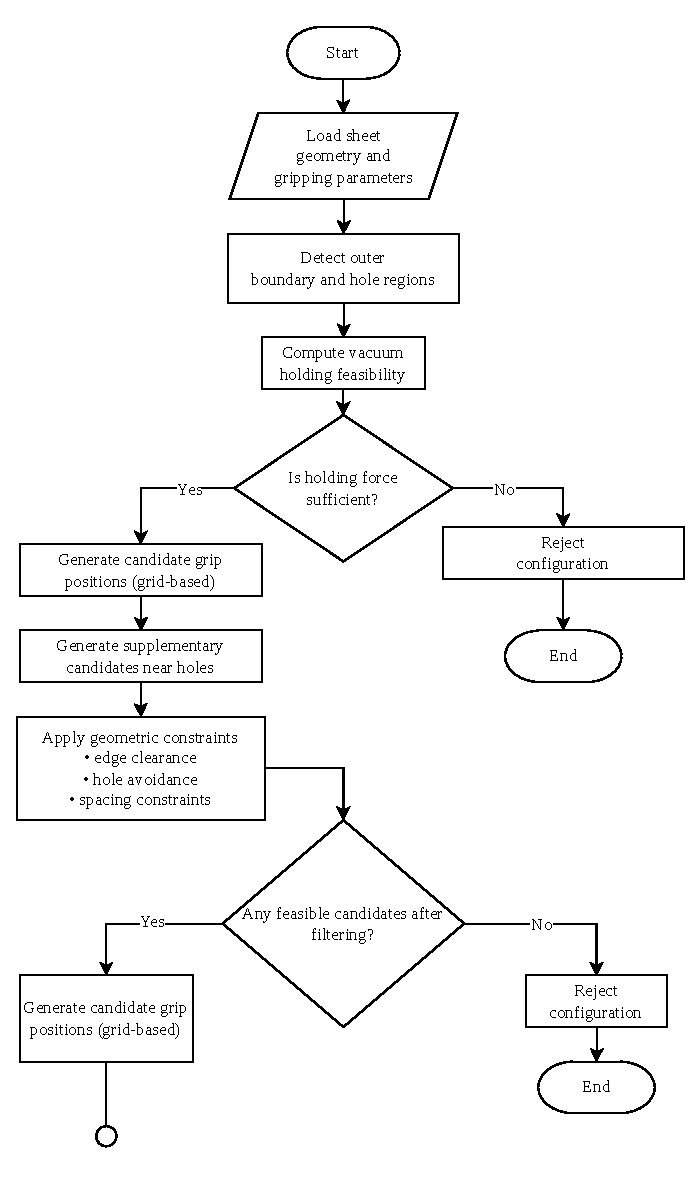
\includegraphics[scale=1]{Flow_Diagrams/grip_planning_workflow_part1.pdf}
        \caption{Input validation, force validation, and candidate generation.}
        \label{fig:grip-planning-flowchart-part1}
    \end{subfigure}
    \caption[Grip planning workflow]{Grip position planning and feasibility validation workflow.}
    \label{fig:grip-planning-flowchart}
\end{figure}

\begin{figure}[p]
    \ContinuedFloat
    \centering
    \setcounter{subfigure}{1}
    \begin{subfigure}{\textwidth}
        \centering
        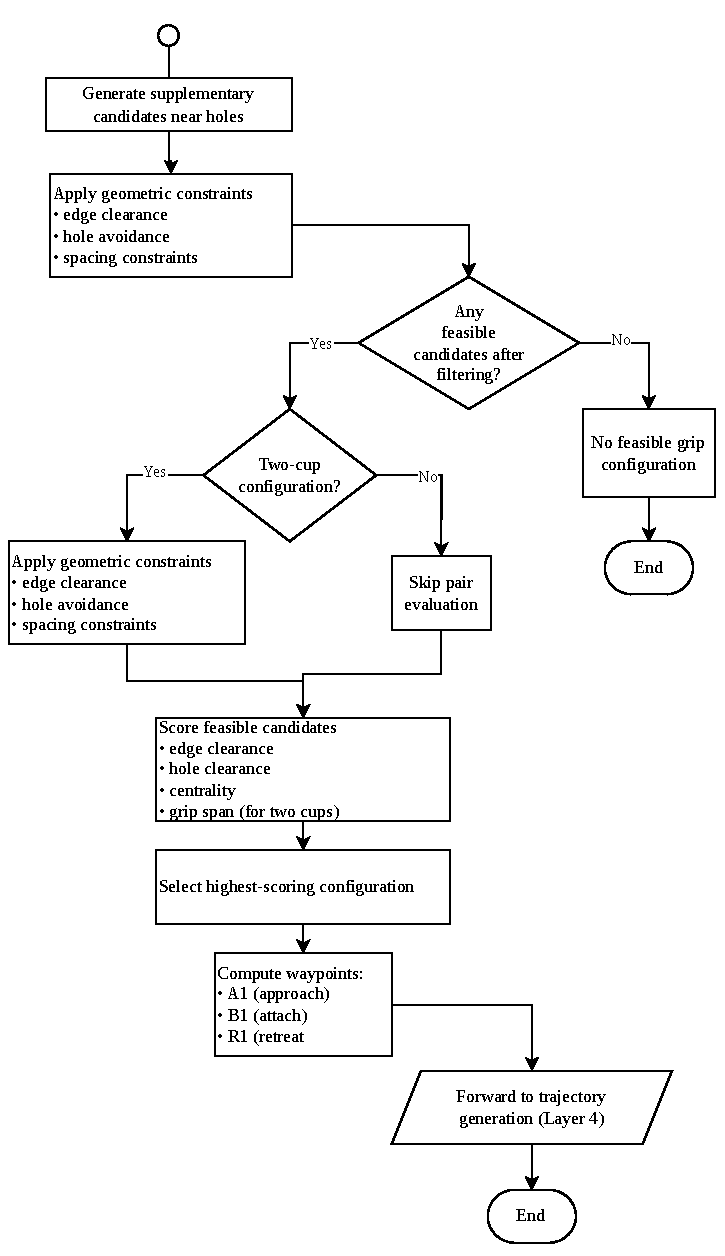
\includegraphics[scale=1]{Flow_Diagrams/grip_planning_workflow_part2.pdf}
        \caption{Constraint filtering, scoring, final grip selection, and waypoint derivation.}
        \label{fig:grip-planning-flowchart-part2}
    \end{subfigure}
    \captionsetup{list=no}
    \caption{Grip position planning and feasibility validation workflow.}
\end{figure}

The selected grip configuration and derived pickup poses define where the gripper must contact the sheet. The following section describes how these planned grasp and release actions are represented during execution.

%%%%%%%%%%%%%%%%%%%%%%%%%%%%%%%%%%%%%%%%%%%%%%%%%%%%%%%%%%%%%%

\section{Gripper State, Regrip, and Opposite-Side Handling}
\label{sec:gripper-control}

After grip planning has selected a feasible suction-cup configuration, the system must convert the planned grasp into a consistent execution state. This requires two actions to remain synchronised: the physical vacuum state of the gripper and the virtual attachment state of the workpiece in the simulation. The input to this stage is the selected grip configuration and the required grasp or release command. The output is a synchronised gripper and workpiece state that can be used by the regrip, flip, and trajectory execution stages.

This separation is necessary because vacuum actuation alone only represents the physical gripping command, while object attachment defines how the sheet follows the robot tool frame in the simulation. If these two states are inconsistent, the simulated workpiece pose may no longer match the intended robot motion, which can lead to incorrect pose propagation and invalid trajectory generation.

\phantomsection\label{sec:vacuum-gripper-digital-io-sequence}
\noindent\textbf{Vacuum gripper digital input and output sequence.}

The vacuum gripper is controlled through digital output signals in the drag\&bot \acs{io} system. One output activates the vacuum, while a second output releases it. These signals are treated as mutually exclusive so that the system does not command vacuum activation and release at the same time.

Control commands are issued via the \texttt{/robot/set\_digital\_ios} interface, which transmits structured \acs{io} instructions specifying the target output and its Boolean state. During a grasp operation, the vacuum is activated before the sheet is attached in the simulation. During release, the vacuum is switched off before the sheet is detached from the robot tool frame. Short guard delays are applied between these actions in the virtual cell to allow state propagation through the runtime interface; for physical deployment, these delays should be tuned to the measured gripper response or replaced by explicit vacuum-state feedback.

\phantomsection\label{sec:kinematic-object-attachment-detachment}
\noindent\textbf{Kinematic object attachment and detachment.}

In the simulation environment, the physical coupling between the gripper and the sheet is represented by kinematic object attachment. When the grasp is confirmed, the sheet object is attached to the robot tool frame so that subsequent robot motion updates the sheet pose consistently. When the gripper releases the sheet, the object is detached and remains at its last known pose.

Attachment is performed using the \texttt{/dnb\_object\_manager/attach} interface without forcing a position override during normal execution. This avoids artificial jumps between the tracked object pose and the simulated state, since the detected sheet pose may not exactly coincide with the instantaneous tool frame pose. Position override is reserved for controlled setup or initialisation cases where explicit pose alignment is required. Detachment is executed using the \texttt{/dnb\_object\_manager/detach} interface within the same reference frame.

The grasp and release procedures therefore follow fixed execution sequences:

\begin{enumerate}
\item Grasp sequence: vacuum ON $\rightarrow$ dwell $\rightarrow$ attach object
\item Release sequence: vacuum OFF $\rightarrow$ dwell $\rightarrow$ detach object
\end{enumerate}

These sequences are centralised so that all modules use the same grasp and release behaviour. This prevents inconsistent conditions where the vacuum state and attachment state do not correspond. With this synchronised handling mechanism defined, the system can safely proceed to regrip planning, opposite-side bending, or trajectory execution.

%%%%%%%%%%%%%%%%%%%%%%%%%%%%%%%%%%%%%%%%%%%%%%%%%%%%

\subsection{Regrip Planning and Execution}
\label{sec:regrip}

Even when a valid pickup orientation and a feasible grip configuration are established, the current grasp may not permit the robot to reach the required bending pose. The input to this stage is the current workpiece pose, selected grip configuration, and target bending pose. The output is either confirmation that direct execution is feasible or a regrip sequence that moves the workpiece into a reachable configuration. This limitation arises when the target configuration lies outside the reachable workspace or when kinematic constraints, such as joint limits or proximity to singularities, prevent a valid motion solution~\cite{lynch2017modern}. To address this implementation limitation within the evaluated virtual cell, the system implements an automatic regrip planning strategy that determines the required reorientation dynamically instead of relying only on predefined handling sequences.

\phantomsection\label{sec:regrip-decision-strategy}
\noindent\textbf{Regrip decision strategy.}

In contrast to conventional approaches based on fixed regrip sequences, the proposed system evaluates a discrete set of candidate workpiece orientations and selects a configuration that satisfies kinematic feasibility. This enables the system to determine both the required orientation and the number of regrip steps automatically.

The candidate set consists of discrete orientation increments corresponding to physically achievable rotations on the orientation table. These candidate orientations, together with the relevant station poses for deposit, re-grasp, retract, and approach motions, are defined through configuration parameters so that the procedure can be reproduced for the same virtual-cell layout. For each candidate orientation, the system performs the following sequence:

\begin{enumerate}
\item Update the workpiece pose according to the candidate orientation
\item Determine a valid pickup orientation using the strategy described in Section~\ref{sec:workpiece-orientation}
\item Compute feasible grip positions using the planner described in Section~\ref{sec:grip-planning}
\item Evaluate kinematic feasibility using inverse kinematics and trajectory validation
\end{enumerate}

A candidate orientation is accepted only when all feasibility conditions are satisfied. The evaluation follows a sequential selection strategy in which candidates are tested in a predefined order, and the first feasible solution is selected. This ensures computational efficiency while maintaining robustness for real-time execution.

The number of required regrip steps is implicitly determined from the difference between the current orientation and the selected feasible configuration. This approach avoids unnecessary intermediate operations while ensuring that the final pose remains reachable and executable within the robot workspace.

The implemented decision process therefore reuses the existing planning pipeline for each candidate orientation. This ensures that regrip selection remains consistent with orientation selection, grip planning, and trajectory generation instead of relying on a separate rule set.

Listing~\ref{lst:regrip-decision} summarises the regrip decision and insertion logic. The direct path is evaluated first; only if it fails does the system evaluate candidate regrip orientations and insert the corresponding handling sequence.

\begin{lstlisting}[caption={Pseudocode for regrip decision and insertion logic.}, label={lst:regrip-decision}]
Evaluate direct trajectory from current grasp to next bending pose
if direct trajectory is feasible then
    continue execution without regrip
else
    for each configured regrip orientation candidate do
        update simulated workpiece pose for candidate orientation
        determine admissible pickup orientation
        compute feasible grip configuration
        validate trajectory from regrip pose to bending pose

        if all checks are feasible then
            select candidate orientation
            insert deposit, release, re-approach, grasp, and return actions
            continue bending sequence
        end if
    end for
end if

if no regrip candidate is feasible then
    trigger controlled stop and operator warning
end if
\end{lstlisting}


\phantomsection\label{sec:regrip-execution-sequence}
\noindent\textbf{Regrip execution sequence.}

Once a feasible orientation has been identified, the system executes a structured regrip sequence to realise the required reorientation. The sequence consists of the following steps:

\begin{enumerate}
\item Transport the workpiece from the bending station approach position to the orientation table deposit position while maintaining the current grasp
\item Release the workpiece through controlled vacuum deactivation and kinematic detachment
\item Move the robot to a retract standoff position to ensure collision-free clearance
\item Re-approach the workpiece at the updated orientation and perform the grasp sequence
\item Repeat the regrip cycle, if further orientation adjustment is required, until a grasp configuration is found from which the gripper can attach to the workpiece and the robot can move directly to the target bending pose
\item Perform the final grasp and return the workpiece to the bending station
\end{enumerate}

Each motion segment is executed using smooth trajectories to minimise dynamic loads on the gripper and ensure stable handling. Intermediate standoff positions provide safe transitions between grasping and releasing operations.

\phantomsection\label{sec:regrip-system-integration-configuration}
\noindent\textbf{System integration and configuration.}

The regrip execution sequence operates within the existing motion framework and uses configuration-defined target positions, including deposit, re-grasp, retract, and approach poses. These parameters define the physical layout of the cell but do not determine the number of regrip steps.

The decision to trigger a regrip is handled by the planning orchestrator, which evaluates feasibility based on orientation admissibility and kinematic constraints. This separation between decision-making and execution ensures modularity and allows the regrip strategy to be extended without modifying the motion execution layer.

Compared to purely configuration-driven approaches, the proposed method improves adaptability by determining the required number of regrip steps dynamically. At the same time, it maintains computational efficiency by evaluating a structured set of candidate orientations rather than performing global optimisation. This balance supports predictable execution within the implemented workflow while keeping the decision process transparent and reproducible.


%%%%%%%%%%%%%%%%%%%%%%%%%%%%%%%%%%%%%%%%%%%%

\subsection{Opposite-Side Bending Workflow}
\label{sec:opposite-side}

After completing all primary-side bending operations, the system evaluates whether additional bends are required on the opposite side of the sheet. The input to this stage is the completed primary-side state and the remaining bend-side requirements. The output is a verified flip sequence that makes the opposite face accessible for the same downstream planning pipeline. These operations cannot be executed directly from the initial pickup configuration, as the required side is not accessible to the press brake tool. Consequently, the workpiece must be reoriented through a controlled flip operation before continuing the bending process.

\phantomsection\label{sec:pre-flip-verification-transition-correction}
\noindent\textbf{Pre-flip verification and transition correction.}

Before initiating the flip sequence, the system verifies that the current sheet pose corresponds to the expected reference configuration. This verification is performed using a wrap-safe six-degree-of-freedom pose comparison, with a positional tolerance of 2~mm and an angular tolerance of 1$^\circ$. These values are configured verification thresholds used in the evaluated virtual cell; they define the accepted deviation before the system triggers a corrective transition rather than manufacturer-specified hardware limits.

This validation step is required because the sheet may have undergone regrip operations during the primary bending sequence. Any deviation from the expected pose would propagate errors into subsequent motion planning stages, leading to incorrect trajectory generation.

If the verification fails, a transition correction step is executed. The system first restores the reference orientation using the strategy described in Section~\ref{sec:workpiece-orientation}. A controlled pickup and repositioning sequence is then performed to re-establish a consistent and verified alignment between the robot and the workpiece.

If the verification is successful, the correction step is omitted and the system proceeds directly to the flip sequence.

\phantomsection\label{sec:sheet-flip-opposite-side-bending-execution}
\noindent\textbf{Sheet flip sequence and opposite-side bending execution.}

The flip operation is performed using a dedicated station within the robotic cell. The workpiece is transferred through two predefined reference positions to achieve a physically feasible reorientation.

First, the robot transports the sheet to the flip station placement position while maintaining the current grasp. The workpiece is then released in a controlled manner. The robot subsequently moves to an intermediate standoff pose and re-approaches the sheet from the opposite side, establishing a new grasp that results in the flipped orientation.

This two-stage transfer is preferred over a direct in-gripper rotation. A direct rotation would require a continuous motion that exceeds the kinematic capabilities of the robot and may violate workspace or collision constraints~\cite{lynch2017modern}.

Following the flip operation, the sheet is aligned such that the previously inaccessible side is oriented towards the press brake tool. The system then applies the same validation pipeline used for primary-side bending, including zone classification, orientation determination, grip position planning, and trajectory generation.

Reusing the same processing pipeline ensures consistent system behaviour across both primary and opposite-side operations. It also avoids the need for separate handling logic, thereby maintaining modularity and reducing system complexity.

Figure~\ref{fig:opposite-face-flip} illustrates the complete opposite-side bending workflow, including pre-flip verification, optional transition correction, flip execution, and subsequent bending operations. The workflow is split into Part~\subref{fig:opposite-face-flip-part1} and Part~\subref{fig:opposite-face-flip-part2} for readability.

After completing all opposite-side bends, any remaining staged operations are executed using the existing handling framework. The system then proceeds to the final unloading sequence.

\begin{figure}[p]
    \centering
    \begin{subfigure}{\textwidth}
        \centering
        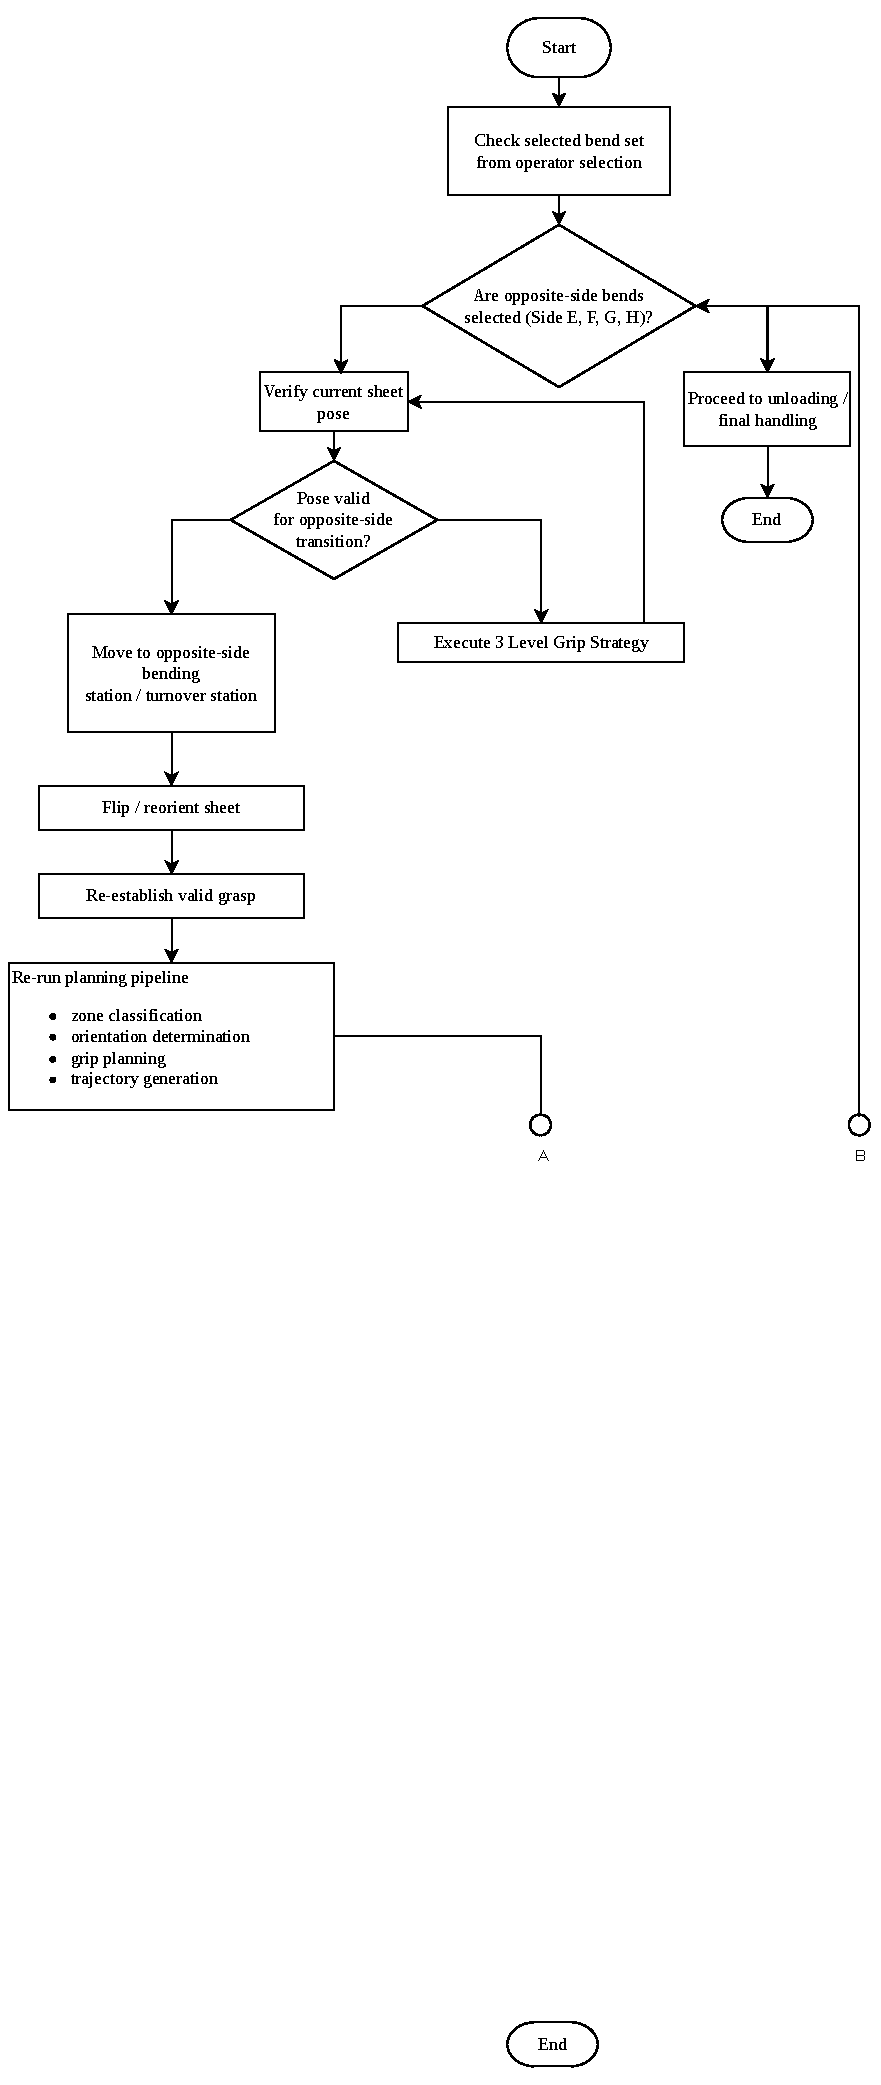
\includegraphics[width=\textwidth,height=0.68\textheight,keepaspectratio]{Flow_Diagrams/opposite_side_flip_workflow_part1.pdf}
        \caption{Pre-flip verification, transition correction, and flip station approach.}
        \label{fig:opposite-face-flip-part1}
    \end{subfigure}
    \caption[Opposite-side flip workflow]{Opposite-side flip workflow enabling access to previously unreachable bending surfaces.}
    \label{fig:opposite-face-flip}
\end{figure}

\begin{figure}[p]
    \ContinuedFloat
    \centering
    \setcounter{subfigure}{1}
    \begin{subfigure}{\textwidth}
        \centering
        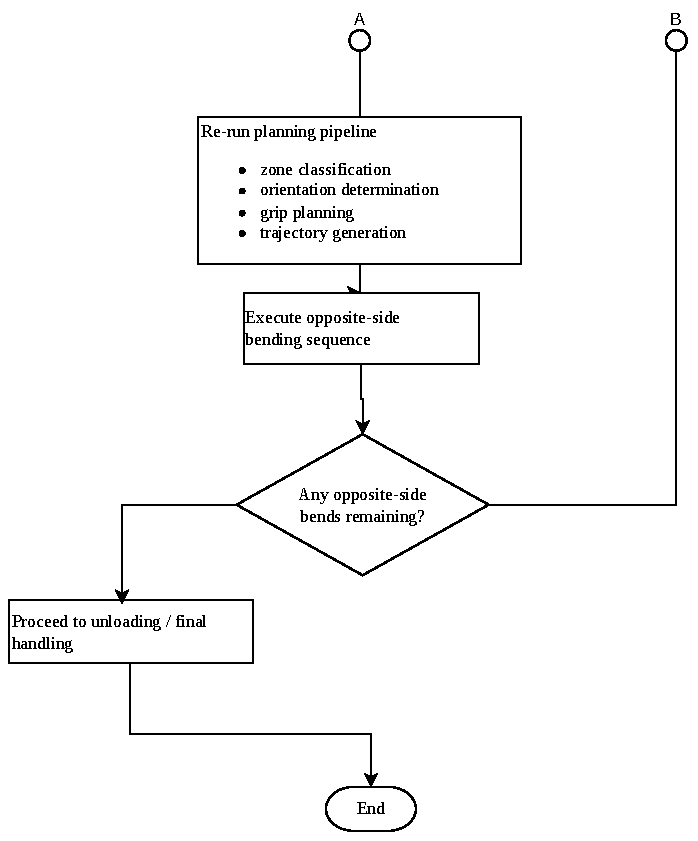
\includegraphics[width=\textwidth,height=0.68\textheight,keepaspectratio]{Flow_Diagrams/opposite_side_flip_workflow_part2.pdf}
        \caption{Opposite-side reorientation, validation, bending continuation, and unloading transition.}
        \label{fig:opposite-face-flip-part2}
    \end{subfigure}
    \captionsetup{list=no}
    \caption{Opposite-side flip workflow enabling access to previously unreachable bending surfaces (continued).}
\end{figure}

%%%%%%%%%%%%%%%%%%%%%%%%%%%%%%%%%%%%%%%%%%%%%%%%%%%%%%%%%%%%%%%%%%%%%%%%%%%%%%%%%%
\section{Trajectory Generation and Execution}
\label{sec:trajectory}

Trajectory generation constitutes the final stage of the planning pipeline, where validated task-level poses are transformed into executable robot motion. The input to this stage is an ordered sequence of \ac{tcp} poses obtained from upstream modules, including grip planning, gripper control actions, regrip handling, and opposite-side operations. The output is a reduced sequence of executable robot motion commands transmitted to the drag\&bot runtime. Each pose defines the desired end-effector position and orientation within the robot world frame.

Rather than executing direct point-to-point transitions, the system constructs a continuous and smooth trajectory composed of intermediate waypoints. This approach ensures kinematic feasibility, reduces dynamic loading, and improves execution stability during sheet handling.

\subsection{Task Sequence Assembly for Execution}
\label{sec:task-sequence-assembly-execution}

Before individual trajectories are generated, the system assembles an ordered task sequence from the validated data produced by the previous modules. The required inputs include the configuration parameters, the current robot pose, the tracked sheet pose, the selected bend side, the validated pickup orientation, the selected grip configuration, the regrip or flip decisions, and the target bending pose. These data define both where the robot must move and which handling actions must be executed between motion segments.

The generated execution program therefore contains motion actions and non-motion actions. Motion actions include approach, attachment, transport, reorientation, bending approach, retreat, and unloading poses. Non-motion actions include vacuum activation and release, as well as kinematic attachment and detachment of the workpiece in the simulation. If direct execution is not feasible, the corresponding regrip cycle is inserted into the sequence. If opposite-side bending is required, the flip sequence is inserted before the remaining bending operations continue through the same planning pipeline.

Each motion action is represented as a start-pose to target-pose segment. The start pose may be the current robot pose, the previous waypoint, a sheet attachment pose, or a pose reached after a regrip or flip operation. The target pose may be a gripping pose, an orientation-table pose, a flip-station pose, a bending pose, or an unloading pose. Between each start and target pose, the trajectory generator automatically inserts intermediate Cartesian waypoints according to the selected path structure and configured motion resolution. These intermediate poses are not manually programmed; they are derived from the validated task poses so that transitions such as robot start to sheet grip, sheet grip to reorientation table, and reorientation table to bending pose can be executed smoothly.

The assembly procedure combines the validated pose data into one ordered action list. Regrip or flip actions are inserted only when required by the feasibility checks. For each motion action, the trajectory generator creates the lift, transfer, and descent structure, interpolates intermediate waypoints, validates feasibility, reduces redundant waypoints, and then passes the resulting motion and handling commands to the drag\&bot runtime.

The waypoint-generation and path-reduction procedure is summarised in Listing~\ref{lst:trajectory-generation}. The listing shows how each motion segment is converted into a dense interpolated trajectory and then reduced before transmission to the robot runtime.

\begin{lstlisting}[caption={Pseudocode for waypoint generation and path reduction.}, label={lst:trajectory-generation}]
for each motion segment in the assembled task sequence do
    define lift pose above start pose using configured safe height
    define transfer pose above target pose
    define descent pose at target task pose

    for each phase between consecutive poses do
        compute path length and required sample count
        interpolate Cartesian position linearly
        interpolate orientation using SLERP
        apply minimum-jerk scaling to interpolation parameter
        append generated waypoint to dense trajectory
    end for

    validate dense trajectory against workspace limits
    remove waypoints below position and rotation change thresholds
    transmit reduced waypoint sequence as linear motion commands
end for
\end{lstlisting}


\subsection{Trajectory Structure and Interpolation}
\label{sec:three-phase-linear-trajectory-structure}

Each start-pose to target-pose segment from the assembled task sequence is generated using a structured three-phase trajectory: lift, lateral transfer, and descent.

In the lift phase, the \ac{tcp} is translated vertically to a predefined safe height to avoid collisions with the workpiece, fixtures, or surrounding environment. In the lateral transfer phase, the robot moves towards the target position while maintaining this clearance height. During this phase, the end-effector orientation is constrained to limit excessive joint rotations and reduce proximity to kinematic singularities. Finally, in the descent phase, the \ac{tcp} is lowered to the target pose, where the required orientation for task execution is fully applied.

To further improve motion feasibility, an intermediate rotation pose is introduced above the target location. This ensures that major orientation adjustments are completed before the final approach, reducing the risk of instability near contact regions.

\phantomsection\label{sec:waypoint-generation-interpolation}
\noindent\textbf{Waypoint generation and interpolation.}

The trajectory between successive poses is generated through interpolation in Cartesian space. For a start pose $\mathbf{T}_s$ and a target pose $\mathbf{T}_t$, the translational component is computed using standard linear interpolation according to Equation~\ref{eq:linear-cartesian-interpolation}~\cite{LibreTextsLinearInterpolation}:

\begin{equation}
\mathbf{p}(\lambda) = (1 - \lambda)\mathbf{p}_s + \lambda \mathbf{p}_t,
\label{eq:linear-cartesian-interpolation}
\end{equation}

where $\lambda \in [0,1]$ is the interpolation parameter.

Rotational interpolation is performed using spherical linear interpolation (SLERP) in quaternion space, which provides smooth and constant-speed rotation between orientations~\cite{Shoemake1985Slerp}.

To ensure smooth velocity and acceleration profiles, the interpolation parameter follows the standard fifth-order minimum-jerk trajectory in Equation~\ref{eq:minimum-jerk-scaling}~\cite{Flash1985MinimumJerk,Sharkawy2021MinimumJerk}:

\begin{equation}
s(u) = 10u^3 - 15u^4 + 6u^5,
\label{eq:minimum-jerk-scaling}
\end{equation}

which guarantees zero velocity and acceleration at the start and end of each motion segment~\cite{Flash1985MinimumJerk}. Such profiles are widely adopted in robotic trajectory planning to achieve smooth and physically consistent motion behaviour~\cite{Gasparetto2012Trajectory}.

By sampling this progression at discrete intervals, the implementation generates intermediate \ac{tcp} waypoints that approximate the continuous trajectory. The same scalar progression is applied to the Cartesian interpolation and to the quaternion-based orientation interpolation so that position and orientation evolve consistently along the segment.

The number of waypoints is determined from the Cartesian path length and a predefined spatial resolution, with a lower bound of two samples. This keeps the trajectory smooth without introducing an unnecessarily dense command sequence.

\subsection{Execution Validation and Path Reduction}
\label{sec:kinematic-mapping-joint-execution}

Each interpolated \ac{tcp} waypoint is mapped to a corresponding robot joint configuration using inverse kinematics. For each waypoint, a feasible solution is selected based on continuity with the previous configuration, avoiding abrupt joint changes and ensuring smooth motion across the trajectory.

As the robot executes the sequence, all joints evolve continuously, resulting in a smooth end-effector motion that closely follows the planned Cartesian path.

\phantomsection\label{sec:workspace-constraints-singularity-handling}
\noindent\textbf{Workspace constraints and singularity handling.}

To ensure execution feasibility, each waypoint is validated against workspace constraints. The \ac{tcp} pose is transformed into the corresponding flange pose, and its position is checked against the allowable workspace limits. If a waypoint exceeds these limits, it is projected onto the nearest feasible boundary.

Singularity avoidance is addressed by restricting orientation changes during the lateral motion phase. Large orientation adjustments are deferred to the approach phase, where the robot operates in a more stable configuration. This reduces the risk of excessive joint velocities and improves overall motion robustness.

\phantomsection\label{sec:motion-execution-path-reduction}
\noindent\textbf{Motion execution and path reduction.}

The interpolation process generates a dense set of waypoints, which may exceed the processing capacity of the robot controller. To address this, a path reduction strategy is applied, retaining only those waypoints that exceed predefined positional or rotational thresholds. This preserves the essential characteristics of the trajectory while reducing communication overhead.

The resulting waypoint sequence is transmitted as a series of linear motion commands, which are executed by the robot controller using blending techniques. This allows smooth transitions between consecutive waypoints without stopping, producing continuous and stable motion.

Overall, the trajectory generation module forms a deterministic transformation pipeline in which validated task-level poses are converted into executable robot motion through interpolation, kinematic mapping, constraint validation, and controlled execution.

%%%%%%%%%%%%%%%%%%%%%%%%%%%%%%%%%%%%%%%%%%%%%%%%%%%%%%%%%%%%%%%%%%%%%%%%%%%%%%%%%%%

The implemented functions are evaluated later through the scenario structure in Chapter~\ref{ch:evaluation-validation}. Table~\ref{tab:ch5-implementation-evaluation-mapping} summarises this connection so that the implementation chapter closes with a clear link between the realised modules, their requirements, and the evidence used in the evaluation.

\begin{table}[htbp]
\centering
\normalsize
\setlength{\tabcolsep}{3pt}
\renewcommand{\arraystretch}{1.08}
\begin{tabularx}{\textwidth}{L{3.8cm} L{3.0cm} Y Y}
\hline
\textbf{Implemented Function} &
\textbf{Related Requirement} &
\textbf{Chapter 6 Evaluation Scenario} &
\textbf{Evidence Type} \\
\hline
Automatic program generation from geometry and configuration &
\acs{fr}-00, \acs{nfr}-01 &
Manual-versus-automated workflow comparison &
Preparation time and execution-ready workflow state \\
\hline
Bend-side selection and workflow branching &
\acs{fr}-02 &
Side~A direct bending and Side~E opposite-side bending &
Scenario-specific generated workflow behaviour \\
\hline
Orientation validation and correction &
\acs{fr}-04 &
Arbitrary initial orientation and position-change scenarios &
Completion classification and planning time \\
\hline
Constraint-based grip planning &
\acs{fr}-06 &
Nominal, geometry-variation, and regrip-required scenarios &
Successful execution or rejected infeasible grips \\
\hline
Automatic regrip planning and execution &
\acs{fr}-03 &
Regrip-required and Side~E scenarios &
Regrip count, execution time, and success rate \\
\hline
Opposite-side flip and reorientation workflow &
\acs{fr}-05 &
Side~E opposite-side workflow &
Success/failure rate and controlled-stop interpretation \\
\hline
Safety validation and controlled-stop handling &
\acs{fr}-07, \acs{nfr}-03, \acs{nfr}-05 &
Failure-prone and constrained-placement scenarios &
Controlled-stop behaviour and warning response \\
\hline
Configuration-driven adaptation and deterministic execution &
\acs{nfr}-02, \acs{nfr}-04, \acs{sr}-01--\acs{sr}-03 &
Geometry variation, position variation, and repeated automated runs &
Scenario averages, repeated-run classification, and virtual runtime execution \\
\hline
\end{tabularx}
\caption{Mapping between implemented functions and the Chapter~6 evaluation evidence.}
\label{tab:ch5-implementation-evaluation-mapping}
\end{table}



\section{Implementation Summary}
\label{sec:implementation-conclusion}

This chapter presented the implementation of the selected Concept~B as a modular planning and execution pipeline for automated press brake sheet metal bending. The system integrates configuration handling, runtime communication, operator input, safety validation, orientation determination, grip planning, regrip and opposite-side handling, and trajectory generation within the drag\&bot-based virtual cell.

A layered architecture was used to keep the implementation testable and maintainable. Each functional component has a defined responsibility, while validation is performed before motion dispatch so that invalid poses, weak grip configurations, and unsafe workspace conditions are detected before execution. The resulting workflow can generate robot programs automatically from configuration data and geometric inputs, reducing the need for manual waypoint definition.

\phantomsection\label{sec:fmea}
\noindent\textbf{Reliability and failure mode analysis.}
After the functional pipeline has been implemented, the remaining question is how the system behaves when individual assumptions or process steps fail. A simplified \ac{fmea}-style scoring convention is therefore used to compare potential failure modes within the robotic bending workflow, evaluate their impact on system performance, and assess the effectiveness of implemented mitigation strategies~\cite{IEC60812_2018}.

The assessment considers three qualitative criteria: severity (S), occurrence (O), and detectability (D). These factors are combined into a Risk Priority Number (RPN) according to the thesis scoring convention defined in Equation~\ref{eq:risk-priority-number}~\cite{IEC60812_2018}:

\begin{equation}
\mathrm{RPN} = S \times O \times D
\label{eq:risk-priority-number}
\end{equation}

Each parameter is assessed using an internal qualitative scale from 1 (low) to 10 (high). Higher RPN values indicate failure modes that require higher-priority mitigation within the scope of this thesis.

\phantomsection\label{sec:identification-failure-modes}
\noindent\textbf{Identified failure modes and mitigations.}

The analysis focuses on critical stages of the execution pipeline, including pickup orientation, grip planning, trajectory execution, regrip handling, and opposite-side operations. The identified failure modes are summarised in Table~\ref{tab:fmea}.

\input{chapters/tables/tab_fmea.tex}

The selected failure modes reflect the most critical dependencies in the system, particularly geometric accuracy, kinematic feasibility, grip reliability, and physical interaction between the robot and the workpiece. Mitigation is handled through fixture pose checks, orientation admissibility limits, grip filtering, vacuum force validation, workspace validation, waypoint reduction, and structured regrip and flip sequences.

The \acs{fmea} results indicate that the most critical risks are associated with pose accuracy, trajectory feasibility, incomplete collision modelling, and the transfer from simulation to physical bending. Pose and feasibility risks are addressed within the implemented system through layered validation, constraint-based planning, and structured motion generation. In contrast, collision-aware deployment and physical bending effects remain documented limitations rather than fully resolved implementation features.

Overall, the system demonstrates a controlled reliability profile within the evaluated simulation conditions. High-severity failure modes are either detected before continuation, converted into controlled stops, or identified as limitations for future physical validation. This indicates that the proposed architecture supports predictable simulated execution while still requiring additional validation before industrial commissioning.

A key contribution of this work lies in the integration of adaptive regrip planning and opposite-side handling within a deterministic execution pipeline. Unlike conventional approaches that rely on predefined sequences, the system dynamically evaluates feasible configurations and determines the required manipulation strategy at runtime. This improves flexibility while maintaining computational efficiency suitable for industrial applications.

The trajectory generation framework further enhances system robustness by combining smooth interpolation techniques with kinematic validation and path reduction strategies. This supports the generation of motions that are executable by the robot controller and stable under the evaluated simulation conditions.

\phantomsection
The detailed requirement compliance matrix\label{sec:requirement-compliance} is provided in Appendix~\ref{app:req-traceability-compliance}, Table~\ref{tab:req-compliance}. It links the functional, non-functional, and software platform requirements to the corresponding implementation components and validation mechanisms. Overall, the implemented system achieves a balance between flexibility, safety, and computational efficiency, demonstrating the feasibility of automated robot program generation within the defined simulation-based scope.
